\documentclass[12pt]{article}
 
\usepackage[margin=1in]{geometry}
\usepackage[pdftex]{hyperref}
\usepackage{amsmath,amsthm,amssymb,caption,graphicx,mathtools,hyperref,enumerate,enumitem}
\usepackage{centernot}
\usepackage{mdframed,cleveref}
\usepackage{bbm}
\usepackage{tikz-cd}


\newmdenv[leftline=false,topline=false]{topright}
\let\proof\relax
\usepackage[utf8]{inputenc}
\usetikzlibrary{positioning}
\newcommand{\n}{\mathbb{N}}
\newcommand{\z}{\mathbb{Z}}
\newcommand{\q}{\mathbb{Q}}
\newcommand{\cx}{\mathbb{C}}
\newcommand{\real}{\mathbb{R}}
\newcommand{\E}{\mathbb{E}}
\newcommand{\V}{\mathbb{V}}
\newcommand{\bb}[1]{\mathbb{#1}}
\let\k\relax
\newcommand{\k}{\mathbf{k}}
\newcommand{\ita}[1]{\textit{#1}}
\newcommand\inv[1]{#1^{-1}}
\newcommand\setb[1]{\left\{#1\right\}}
\newcommand{\vbrack}[1]{\langle #1\rangle}
\newcommand{\determinant}[1]{\begin{vmatrix}#1\end{vmatrix}}
\newcommand{\abs}[1]{\left\vert #1 \right\vert}
\DeclareMathOperator{\Id}{Id}


\hypersetup{
	colorlinks,
	linkcolor=blue
}
 
 \renewcommand*\contentsname{Continguts}

\newtheoremstyle{break}% name
{}%         Space above, empty = `usual value'
{}%         Space below
{}% Body font
{}%         Indent amount (empty = no indent, \parindent = para indent)
{\bfseries}% Thm head font
{}%        Punctuation after thm head
{\newline}% Space after thm head: \newline = linebreak
{#1 #2 \normalfont #3}%         Thm head spec

\newtheoremstyle{breakthm}% name
{}%         Space above, empty = `usual value'
{}%         Space below
{}% Body font
{}%         Indent amount (empty = no indent, \parindent = para indent)
{\bfseries}% Thm head font
{}%        Punctuation after thm head
{\newline}% Space after thm head: \newline = linebreak
{#1 \normalfont #3 (#2)\addcontentsline{toc}{subsubsection}{#1 #3}}%         Thm head spec
\newtheoremstyle{normal}% name
{}%         Space above, empty = `usual value'
{}%         Space below
{}% Body font
{}%         Indent amount (empty = no indent, \parindent = para indent)
{\bfseries}% Thm head font
{}%        Punctuation after thm head
{5pt plus 1pt minus 1pt}% Space after thm head: \newline = linebreak
{#1 #2 \normalfont #3}%         Thm head spec

\theoremstyle{normal}
\newtheorem{lema}{Lema}[subsection]
\newtheorem{obs}[lema]{Observació}

\theoremstyle{break}
\newtheorem{prop}[lema]{Proposició}
\newtheorem{properties}[lema]{Propietats}
\newtheorem*{proof}{Demostració}
\newtheorem{defi}[lema]{Definició}
\newtheorem{col}[lema]{Corol·lari}
\newtheorem{ej}[lema]{Exercici}
\newtheorem{example}[lema]{Exemple}

\theoremstyle{breakthm}
\newtheorem{thm}[lema]{Teorema}
\newtheorem{defiImp}[lema]{Definició} %Pq surti al índex



\setcounter{section}{1}

 
\begin{document}
\date{}
\setlength{\parindent}{0pt}

\title{Teoria de la Probabilitat}
\author{Ferran Arqué}
 
\maketitle

\tableofcontents

\setcounter{section}{0}

\newpage
\section{Espais de Probabilitat}

\subsection{Definició axiomàtica d'espai de probabilitat}

\begin{defi}
  Un \textbf{espai de probabilitat} és un espai de mesura $(\Omega, \mathcal{A}, p)$, tal que $p(\Omega) = 1$.
  \begin{itemize}
      \item $\Omega$ s'anomena \textbf{espai mostral}.
      \item $\mathcal{A}$ se l'anomena \textbf{conjunt d'esdeveniments} o \textbf{successos}.
      \item $p$ se l'anomena \textbf{funció de probabilitat}.
  \end{itemize}
\end{defi}

\begin{obs}
  $\mathcal{A} \subseteq \mathcal{P}(\Omega)$ és una $\sigma$-àlgebra: \\
  $\sigma1)$ $\varnothing \in \mathcal{A}$ \\
  $\sigma2)$ $A \in \mathcal{A} \iff \overline{A} \in \mathcal{A}$ \\
  $\sigma3)$ Si $\setb{A_{n}}_{n\geq1}$ és una seqüència de successos en $\mathcal{A} \implies \bigcup\limits_{n\geq1}A_{n} \in \mathcal{A}$
\end{obs}

\begin{obs}
  Recordem que $p$ és una mesura i, per tant: \\
  $p1)$ $p(\varnothing) = 0$ \\
  $p2)$ $\forall A \in \mathcal{A},\, p(A)\geq0$ \\
  $p3)$ Si $\setb{A_{n}}_{n\geq1}$ és una seqüència de successos en $\mathcal{A}$ disjunts 2 a 2 $(A_{i}\cap A_{j} = \varnothing \, si \, i \not =j)$, aleshores 
  \[
    p\bigg(\bigcup\limits_{n\geq1}A_{n}\bigg) = \sum_{n\geq1}p(A_{n})
  \]
\end{obs}

Vegem les primeres propietats dels espais de probabilitat:

\begin{prop}
  Per un espai de probabilitat $(\Omega, \mathcal{A}, p)$ es compleix que: \\
  (i) $A\in\mathcal{A} \implies p(\overline{A}) = 1-p(A)$ \\
  (ii) Si $A, B \in \mathcal{A},\, A \subseteq B \implies p(A)\leq p(B)$ \\
  (iii) Si $A_{1},\ldots,A_{r} \in \mathcal{A}, \, i \, A_{i}\cap A_{j} \not= \varnothing \, (i\not= j)$, aleshores $p\bigg(\bigcup\limits_{i=1}^{r}A_{i} \bigg) = \sum\limits_{i=1}^{r}p(A_{i})$ \\
  (iv) Si $A,B \in \mathcal{A}, \, A\subseteq B \implies p(B-A) = p(B)-p(A)$\\
  (v) Successions monòtones: 
  \[
    \hspace{-2.5cm}\text{a) Si } A_{1} \subseteq A_{2} \subseteq A_{3} \subseteq \ldots \subseteq A_{i} \in \mathcal{A} \implies p\bigg(\bigcup\limits_{n\geq1}A_{n}\bigg) = \lim_{n\to\infty}p(A_{n})
  \]
  \[
    \hspace{-2.5cm}\text{b) Si } A_{1} \supseteq A_{2} \supseteq A_{3} \supseteq \ldots \supseteq A_{i} \in \mathcal{A} \implies p\bigg(\bigcap\limits_{n\geq1}A_{n}\bigg) = \lim_{n\to\infty}p(A_{n})
  \]
\end{prop}

\newpage

Si ara tenim un espai de probabilitat $(\Omega, \mathcal{A},p)$, i successos $A_{1}, A_{2}, \ldots, A_{i}$ en general \underline{no} disjunts, aleshores \underline{no} és cert que  $p\bigg(\bigcup\limits_{i=1}^{r}A_{r} \bigg) = \sum\limits_{i=1}^{r}p(A_{i})$. En aquest cas, tenim la següent fita:
\begin{lema}[(Fita de la unió)] \-\\
  Siguin $A_{1}, A_{2}, \ldots, A_{r}$ successos en $(\Omega, \mathcal{A},p)$, aleshores $$p\bigg(\bigcup\limits_{i=1}^{r}A_{i} \bigg) \leq \sum\limits_{i=1}^{r}p(A_{i})$$
\end{lema}

\begin{thm}[(Desigualtats de Bonferroni)]
  Siguin $A_{1}, \ldots, A_{r}$ successos en $(\Omega, \mathcal{A}, p)$. 
  Denotem per $I\subseteq \setb{1,\ldots,r} \colon = [r]$, \\
  \[
    A_{I} = \bigcap\limits_{i\in I}A_{i}
  \]
  \[
    S_{k} = \sum_{\substack{I\subseteq[r] \\ \abs{I}=k}}p(A_{I})
  \]
  Aleshores, si: \\
  1) t és parell, $p\bigg(\bigcup\limits_{i=1}^{r} A_{i}\bigg)\geq \sum\limits_{i=1}^{t}(-1)^{i+1}\cdot S_{i}$\\\\
  2) t és senar, $p\bigg(\bigcup\limits_{i=1}^{r} A_{i}\bigg)\leq \sum\limits_{i=1}^{t}(-1)^{i+1}\cdot S_{i}$
\end{thm}

\begin{example}

\end{example}

\newpage

\subsection{Probabilitat condicionada}
\begin{defi}
  Sigui $(\Omega, \mathcal{A}, p)$ un espai de probabilitat , i $B \in \mathcal{A}$ amb $p(B) > 0$. \\
  Per $A \in \mathcal{A}$, la \textbf{probabilitat condicionada} de A amb B és:
  \[
    p(A\mid B) = \frac{p(A\cap B)}{p(B)}
  \]
\end{defi}

\begin{obs}
  $p(A \mid B)$ mesura la probabilitat de que el succés $A$ ocorri sabent que $B$ ha succeït.
\end{obs}

\begin{obs}
  Si prenem
  \[
  \begin{aligned}
      P_{B} \colon \mathcal{A} &\to \real \\
      A &\mapsto P_{B}(A) = P(A\mid B)
  \end{aligned}
  \]
  Aleshores $P_{B}$ és una funció de probabilitat sobre $\Omega, \mathcal{A}$ \\
  De fet, si definim $\mathcal{A}_{B} = \setb{A\cap B\colon A\in\mathcal{A}}$, aleshores $\mathcal{A}_{B}$ és una $\sigma$-àlgebra i $P_{B}$ també defineix una probabilitat sobre $(\Omega, \mathcal{A}_{B})$.
\end{obs}

\begin{prop}
  Siguin $A_{1}, \ldots, A_{r} \in \mathcal{A}$, tals que $p(A_{i}) > 0, \, A_{i}\cap A_{j} = \varnothing \text{ si } i \not= j$ i $\bigcup\limits_{i = 1}^{r}A_{i} = \Omega \\ \quad (\setb{A_{i}}_{i=1}^{r}$ és una partició de $\Omega)$ \\
  
  (i) \underline{Teorema de la probabilitat total}: $\forall A \in \mathcal{A}, p(A)=\sum\limits_{i=1}^{r}p(A \mid A_{i})\cdot p(A_{i})$. \\
  (ii) \underline{Fórmula de Bayes}: si $A \in \mathcal{A}, \, p(A) > 0,$
  \[
    p(A_{j} \mid A) = \frac{p(A\mid A_{j})\cdot p(A_{j})}{\sum\limits_{i=1}^{r}p(A \mid A_{i})\cdot p(A_{i})}
  \]
\end{prop}

Molts cops serà més senzill calcular probabilitats condicionades. Vegem un exemple:
\begin{example}[(La ruïna del jugador)]
  Partim d'un capital de $k$ unitats $(k \geq 0)$ i volem aconseguir un capital de $N$ unitats $(N\geq k)$ de la següent forma: \\
  Llancem una moneda equilibrada, guanyant (surt cara) o perdent (surt creu) una unitat amb probabilitat $\frac{1}{2}$. El joc acaba si: 
  \begin{enumerate}
      \item Ens quedem sense capital.
      \item Assolim un capital igual a N
  \end{enumerate}
  Calcularem la probabilitat de perdre. \\
  No és bona idea intentar codificar tots els casos possibles i sumar les seves probabilitats \\ (nº tirades $\to \infty$). \\\\
  
  Anem a resoldre el problema usant el teorema de la probabilitat total. \\
  $A_{k} = $ "el jugador, amb capital inicial igual a $k$, s'arruïna" (Volem calcular $p(A_{k})$). \\
  Escrivim $p(A_{k}) = p_{k}$. Aleshores $p_{0} = 1, \, p_{N} = 0$. \\
  Definim $B =$ "la primera tirada de la moneda és cara". Aleshores $B$ i $\overline{B}$ defineixen una partició de $\Omega$. \\
  Usem el teorema de probabilitat total:
  \[
    \begin{rcases}
        p(A_{k}) &= p(A_{k} \mid B)p(B) + p(A_{k}\mid \overline{B})p(\overline{B}) \\
        &= p(A_{k}\mid B)\cdot\frac{1}{2} + p(A_{k}\mid\overline{B})\cdot\frac{1}{2} \\
        &= \frac{1}{2} \cdot\Big( \underbrace{p(A_{k}\mid B)}_{p(A_{k+1})} + \underbrace{p(A_{k}\mid\overline{B})}_{p(A_{k-1})}\Big)
    \end{rcases} p_{k} = \frac{1}{2}(p_{k+1} + p_{k-1}); \quad p_{0} = 1, \, p_{N} = 0
  \]
  
  Resolent la recurrència tenim: 
  \[
    p_{k} = 1 - \frac{k}{N}
  \]
  Si $k \in o(N)$, aleshores assimptòticament el jugador s'acabarà arruïnant.
\end{example}

\subsection{Independència}

\begin{defi}
  Dos successos $A$ i $B$ (del mateix espai $(\Omega, \mathcal{A}, p)$) són \textbf{independents} si $p(A\cap B) = p(A)\cdot p(B)$.
\end{defi}

\begin{obs}
  \begin{itemize}
      \item []
      \item Si $p(B) > 0$, $A$ i $B$ independents $\iff p(A\mid B)=p(A)$
      \item El successos $\varnothing$ i $\Omega$ són independents amb qualsevol altre succés B
      \item Si $A$ i $B$ són independents, $A$ i $\overline{B}$ també. (De fet tenim que $A$ i $B$ són independents $\iff \overline{A}$ i $\overline{B}$ són independents).
  \end{itemize}
\end{obs}

\begin{defi}
  Donada una família de successos $\setb{A_{i}}_{i\in I}$, es diu que és \textbf{independent} si:
  \[
    \forall J \subseteq I \text{ amb } \abs{J} < \infty \text{, es té: } p\bigg(\bigcap\limits_{j\in J}A_{j}\bigg) = \prod_{j\in J}p(A_{j}) 
  \]
\end{defi}

\begin{obs}
  Donats $\setb{A_{i}}_{i = 1, \ldots, r}$ successos, poden ser independents dos a dos però no com a conjunt.
\end{obs}

\newpage

\subsection{Espai producte}

Donats dos espais de probabilitat $(\Omega_{1}, \mathcal{A}_{1}, p_{1})$ i $(\Omega_{2}, \mathcal{A}_{2}, p_{2})$, volem combinar-los en un sol espai amb espai mostral $\Omega_{1}\times\Omega_{2}$. \\
Això ja ho hem fet en el cas discret, però en general:
\begin{itemize}
    \item Prenem com a espai mostral $\Omega_{1}\times\Omega_{2}$
    \item Prenem com a $\sigma$-àlgebra $\sigma(\mathcal{A}_{1}\times\mathcal{A}_{2})$ (la més petita $\sigma$-àlgebra que conté $\mathcal{A}_{1}\times\mathcal{A}_{2}$).
    \item Com definim $p$ a $(\Omega_{1}\times\Omega_{2}, \mathcal{A}_{1}\times\mathcal{A}_{2})$? \\ Voldríem que $p(A_{1}\times A_{2}) = p(A_{1})\cdot p(A_{2}) \quad \forall A_{i} \in \mathcal{A}_{i}$. Per definir $p$ necessitarem el següent teorema:
\end{itemize}

\begin{thm}[(d'extensió o de Carathéodory)]
  Sigui $p_{0}$ una funció de probabilitat en una àlgebra $\mathcal{A}_{0}$. Sigui $\mathcal{A} = \sigma(\mathcal{A}_{0})$. \\
  Aleshores $p_{0}$ es pot extendre a una funció de probabilitat $p$ sobre $\mathcal{A}$ que coincideix amb $p_{0}$ en $\mathcal{A}_{0}$. A més, $p$ és única.
\end{thm}

En el nostre cas, quina àlgebra agafem? 
\[
    \underbrace{(\mathcal{A}_{1}\times\mathcal{A}_{2})^{*}}_{\mathcal{A}_{0}} = \text{ totes les unions finites d'elements de } \mathcal{A}_{1}\times\mathcal{A}_{2}.
\]
Es comprova que $\sigma((\mathcal{A}_{1}\times\mathcal{A}_{2})^{*}) = \sigma(\mathcal{A}_{1}\times\mathcal{A}_{2})$ i apliquem el teorema.

\subsection{Lema de Borel-Cantelli}

Sigui $(\Omega, \mathcal{A}, p)$ un espai de probabilitat.

\begin{defi}
  Donada $\setb{A_{n}}_{n\geq 1}$ un successió de successos, 
  \[
    \text{lim sup } A_{n} = \bigcap\limits_{n=1}^{\infty}\bigcup\limits_{k=n}^{\infty}A_{k}
  \]
  \[
    \text{lim inf } A_{n} = \bigcup\limits_{n=1}^{\infty}\bigcap\limits_{k=n}^{\infty}A_{k}
  \]
\end{defi}

\begin{obs}
  Tant \textit{lim sup} $A_{n}$ com \textit{lim inf} $A_{n}$ són successos.
\end{obs}

\begin{defi}
  Si $\setb{A_{n}}_{n\geq 1}$ és una successió de successos amb $lim \, sup\, A_{n} = lim\, inf\, A_{n}$, aleshores $\setb{A_{n}}_{n\geq 1}$ té \textbf{límit} i l'escriurem $lim A_{n} = lim \, sup \, A_{n}$.
\end{defi}

\newpage

\begin{properties}
  Sigui $\setb{A_{n}}_{n\geq 1}$ una successió de successos: \\\\
  (i) $lim \, sup \, A_{n} = \setb{\omega \in \Omega \colon \omega \text{ pertany a un nombre infinit de } A_{i}'s}$ \\\\
  (ii) $lim \, inf \, A_{n} = \setb{\omega \in \Omega\, \colon \exists \, m = m(\omega) \text{ tal que } \omega\in A_{r} \text{ si } r \geq m(\omega)}$ \\\\
  (iii) $lim \, inf\, A_{n} \subseteq lim\, sup \, A_{n}$ \\
\end{properties}

Si ara $lim \, sup\, A_{n} = lim\, inf\, A_{n} = lim A_{n}$, podem intercanviar $lim$ amb $p$:

\begin{prop}
  Sigui $\setb{A_{n}}_{n\geq 1}$ una successió de successos amb $lim A_{n} = A$. Aleshores, $p(A) = lim \, p(A_{n})$. \\
\end{prop}

El següent lema ens dóna condicions suficients molt senzilles per a calcular $p(lim \, sup \, A_{n})$.

\begin{lema}[(Borel-Cantelli)]
  \- \\
  Sigui $(\Omega, \mathcal{A}, p)$ un espai de probabilitat i $\setb{A_{n}}_{n\geq 1}$ una successió de successos. Aleshores: \\\\
  
  (i) Si $\sum\limits_{n\geq 1}p(A_{n}) < \infty \implies p(lim \, sup \, A_{n}) = 0$ \\\\
  
  (ii) Si els $\setb{A_{n}}_{n\geq 1}$ són successos independents i $\sum\limits_{n\geq 1}p(A_{n}) = \infty \implies p(lim \, sup \, A_{n}) = 1$
\end{lema}

\begin{obs}
  No podem treure la condició d'independència de (ii). \\
  Si prenem $A_{n} = E$ succés amb $0 < p(E) < 1$, aleshores $\sum\limits_{n\geq 1}p(A_{n}) = \sum\limits_{n\geq 1}p(E)$, els $A_{n}$ \underline{no} són independents i  $p(lim \, sup \, A_{n}) = p(E) < 1$.
\end{obs}

\newpage
\section{Variables Aleatòries}
\subsection{Definició de variable aleatòria. Llei d'una v.a.}
Sigui $(\Omega, \mathcal{A}, \beta)$  un espai de probabilitat. Volem estudiar funcions de $\Omega$ amb imatge en $\real$.

\begin{defi}
  Una \textbf{variable aleatòria} és una funció $X\colon \Omega \to \real$ tal que per tot borelià B 
  $\in \mathcal{B}$, $\inv{X}(B) \in \mathcal{A}$. \\
  
  Per tant, una variable aleatòria és una funció mesurable entre els espais de mesura $(\Omega, \mathcal{A}, p)$ i $(\real, \mathcal{B}, \lambda)$.
\end{defi}

\begin{example}
  (1) Les funcions constants són variables aleatòries: \\
    \[
    \begin{aligned}
      X \colon \Omega &\to \real \\
      \omega &\mapsto c
    \end{aligned}
    \qquad \text{Si prenem } B \in \mathcal{B} \text{, } \inv{X}(B) =
    \begin{cases}
			\varnothing \quad \text{si c} \notin B\\
			\Omega \quad \text{si c} \in B
    \end{cases}
    \]
  \\
  
  (2) \textbf{Variables aleatòries indicadores}: 
    \[
    \hspace{-3.5cm}\text{Sigui A}  \in \mathcal{A}\text{, definim }\mathbbm{1}_{A}\colon \Omega \to \real \text{ on } \mathbbm{1}_{A}(\omega) = 
    \begin{cases}
			0 \quad \text{si } \omega \notin A\\
			1 \quad \text{si } \omega \in A
    \end{cases}\\
    \]
    \[
    \hspace{-3.5cm}\text{Aleshores, } B \in \mathcal{B}, \inv{\mathbbm{1}_{A}}(B) = 
    \begin{cases}
			\varnothing \quad \text{si } \setb{0, 1} \nsubseteq B\\
			A \quad \text{si } 1 \in B, \quad 0\notin B\\
			\overline{A} \quad \text{si } 1 \notin B, \quad 0 \in B\\
			\Omega \quad \text{si } \setb{0, 1} \nsubseteq B
    \end{cases}\\
    \]
    \\
    
    (3) Si X i Y són v.a., aleshores $X + Y$, $X\cdot Y$, $\abs{X}$, etc. són v.a. \\
    \- \hspace{0.5cm}En general, si $g\colon \real^{2} \to \real$ és una funció mesurable, aleshores g(X,Y) és una v.a.\\
\end{example}

Estem dient que $\forall B \in \mathcal{B}$, $\setb{\omega \in \Omega \colon X(\omega) \in B}$ és un succés i, per tant, podem calcular $P(\setb{\omega \in \Omega \colon X(\omega) \in B}) \equiv P(X \in B)$.\\

\begin{example}
  $P(X\leq 1) = P(\setb{\omega \in \Omega \colon X(\omega) \in (-\infty, 1)})$\\
\end{example}

Les v.a. permeten traslladar l'estructura d'espai de probabilitat de $(\Omega, \mathcal{A}, p)$ en $(\real, \mathcal{B})$, donant lloc a mesures que no provenen de la mesura de Lebesgue.\\

\newpage

\begin{defi}
  Siguin $(\Omega, \mathcal{A}, p)$ un espai de probabilitat i X una v.a. \\
  La \textbf{mesura de probabilitat induïda} per X és una mesura de probabilitat sobre $(\real, \mathcal{B})$ definida per
  \[
    \begin{aligned}
      p_{X} \colon \mathcal{B} &\to \real \\
      B &\mapsto p_{X} = P(\setb{\omega \in \Omega \colon X(\omega) \in B})
    \end{aligned}
  \]
  \\
\end{defi}

\begin{obs}
  $(\real, \mathcal{B},p_{X})$ és un espai de probabilitat.
\end{obs}

De teoria de la mesura, és equivalent veure que [$\forall B \in \mathcal{B}, \quad \inv{X}(B) \textit{ és de } \mathcal{A}$] a veure que [\textit{l'antiimatge de qualsevol interval} $\in \mathcal{A}$].\\\\
Per tant, per saber si una funció és una v.a. només cal veure si l'antiimatge dels intervals són de $\mathcal{A}$.\\

La següent definició dóna una funció en $\real$ que codifica molta informació de X:

\begin{defi}
  Donada X v.a., la \textbf{funció de distribució de probabilitat} de X és:
  \[
    \begin{aligned}
      F_{X} \colon \real &\to [0,1] \\
      x &\mapsto P(X \leq x)
    \end{aligned} 
  \]
\end{defi}

\begin{properties}
  (i) Si $x_{1} \leq x_{2} \implies F_{X}(x_{1}) \leq F_{X}(x_{2})$\\
  \[
  \hspace{-9.4cm}\text{(ii) }\lim_{x\to -\infty} F_{X}(x) = 0 \text{ ,  } \lim_{x\to+\infty} F_{X}(x) = 1
  \]
  (iii) $F_{X}(x)$ és contínua per la dreta: $\forall x, \lim_{h\to0^{+}}F_{X}(x+h) = F_{X}(x)$
\end{properties}

\begin{obs}
  \begin{itemize}
      \item []
      \item $P(X > x) = 1 - P(X\leq x) = 1 - F_{X}(x)$
      \item $P(x_{1} < X \leq x_{2}) = P(X \leq x_{2}) - P(X \leq x_{1}) = F_{X}(x_{2}) - F_{X}(x_{1})$
  \end{itemize}
\end{obs}

\begin{obs}
  Les propietats (i), (ii), (iii) de $F_{X}(x)$ són de fet suficients.\\
  Si una funció $F(x)$ satisfà (i), (ii), (iii), aleshores és funció de probabilitat d'una variable aleatòria.
\end{obs}
\newpage
\subsection{Moments d'una v.a.  Desigualtats de Markov i Chebyshev}

Siguin $(\Omega, \mathcal{A}, p)$ uns espai de probabilitat i X una v.a.\\
\begin{defi}
  L'\textbf{esperança} de X és: 
  \[
  \E[X] = \int_{\Omega}X dp = \int_{\real} x \, dp_{X}
  \]
  \\
  Més en general, si $f\colon \real \to \real$ és una funció mesurable, 
  \[
    \E[f(x)] = \int_{\Omega}f(x) dp = \int_{\real} f(x) \, dp_{X}
  \]
\end{defi}

\begin{obs}
  De teoria de la mesura, cal recordar que una funció $g$ és integrable sii $\abs{g}$ ho és
  (En general, $\E[f(x)]$ està definida sii $\E[\abs{f(x)}]<+\infty$). \\
\end{obs}

Si particularitzem $f$:

\begin{defi}
  $f(x) = X^{r} \implies \E[X^{r}]$ és el \textbf{moment r-èssim}.
\end{defi}

\begin{defi}
  Si $\E[X] = p < +\infty$, $\E[(X-p)^{r}]$ és el \textbf{moment normalitzat r-èssim}.\\\\
  En particular, si r = 2, $\E[(X-p)^{2}] = \mathbbm{V}ar[X]$ és la \textbf{variància} de $X$.
\end{defi}

\begin{defi}
  Si $f(x) = x(x-1)\ldots(x-r+1) \implies \E[f(x)] = \E[(X)_r]$ és el \textbf{moment factorial r-èssim}.
\end{defi}

\begin{prop}[(Propietats de l'esperança i la variància)]
  \begin{itemize}
      \item []
      \item Si $c$ és la v.a. constant, $\E[c] = c$ i $\mathbbm{V}ar[c] = 0$
      \item \underline{Linealitat}: si $a, b \in \real$ i $X, Y$ v.a., $\E[aX + bY] = a\E[X] + b\E[Y]$
      \item $A \in \mathcal{A}, X = \mathbbm{1}_{A}$, $\E[\mathbbm{1}_{A}] = P(A)$
      \item $\abs{\E[X]} \leq \E[\abs{X}]$
      \item $\mathbbm{V}ar[c\cdot X] = c^{2}\cdot \mathbbm{V}ar[X]$
      \item $\mathbbm{V}ar[c+X] = \mathbbm{V}ar[X]$
      \item $\mathbbm{V}ar[X] = \E[X^{2}] - (\E[X])^{2}$
  \end{itemize}
\end{prop}

\newpage

\begin{obs}
  Si $\E[\abs{X}^{p}] < +\infty$, aleshores podem utilitzar tots els resultats de teoria dels espais $L_{p}$. Així doncs tenim les següents conseqüències:
  
  \begin{itemize}
      \item \underline{Hölder}: $p, q > 0$, $\frac{1}{p} + \frac{1}{q} = 1, \, \E[\abs{X}^{p}] < +\infty, \E[\abs{Y}^{q}] < +\infty \\ \- \hspace{1.25cm}\implies \E[\abs{XY}] \leq \E[\abs{X}^{p}]^{\frac{1}{p}}\cdot \E[\abs{Y}^{q}]^{\frac{1}{q}} \quad (\E[\abs{XY}]^{pq} \leq \E[\abs{X}^{p}]^{q}\cdot \E[\abs{Y}^{q}]^{p})$
      
      \item \underline{Cauchy-Schwartz}: si $\E[X^{2}], \E[Y^2] < +\infty$, aleshores $\E[XY]^{2} \leq \E[X^{2}]\cdot \E[Y^{2}]$
      \item \underline{Minkowski}: si $\E[\abs{X}^{p}], \E[\abs{Y}^{p}] < +\infty \implies \E[\abs{X+Y}^{p}]^{\frac{1}{p}} \leq \E[\abs{X}^{p}]^{\frac{1}{p}} + \E[\abs{Y}^{p}]^{\frac{1}{p}}$
  \end{itemize}
\end{obs}

\begin{thm}[(Desigualtat de Markov)]
  Sigui $X$ un v.a. que pren valors positius i $a > 0$. Aleshores: \\
  \[
    P(X \geq a) \leq \frac{\E[X]}{a}
  \]
\end{thm}

El següent resultat dóna estimacions quantitatives de quant es dispersa una v.a. en relació a la seva esperança:

\begin{thm}[(Desigualtat de Chebyshev)]
  Sigui X una v.a. en $(\Omega, \mathcal{A}, p)$ amb $\E[X], \V ar[X] < +\infty$. Aleshores, $\forall k > 0$
  \[
    P(\abs{X-\E[X]}\geq k\cdot \V ar[X]^{\frac{1}{2}}) \leq \frac{1}{k^{2}}
  \]
  També es pot escriure:
  \[
    P(\abs{X-\E[X]}\geq k) \leq \frac{\V ar[X]}{k^{2}}
  \]
\end{thm}

%\newpage
\subsection{Vectors de variables aleatòries. Independència de v.a.}

Donat un espai de probabilitat $(\Omega, \mathcal{A}, p)$ considerem les v.a. $X_{1}, \ldots, X_{n}$.  Cadascuna d'elles defineix una distribució de probabilitat sobre $\real$. \\
Aleshores podem considerar el vector $(X_{1}, \ldots, X_{n})\colon \Omega \to \real^{n}$. 

\begin{defi}
  Un vector $(X_{1}, \ldots, X_{n})\colon \Omega \to \real^{n}$ és un \textbf{vector de variables aleatòries} (o una v.a. multidimensional), si per tot $B \in \mathcal{B}_{n}$ (Borelians en $\real^{n}$), $\inv{(X_{1}, \ldots, X_{n})}(B) \in \mathcal{A}$. \\
  
  Com $\Pi_{i}\colon \real^{n} \to \real$ (projecció en la i-èssima component) és una funció mesurable, aleshores 
  \[
  \begin{aligned}
      \Pi_{i}(X_{1}, \ldots, X_{n}) \colon \Omega &\xrightarrow{(X_{1}, \ldots, X_{n})} \real^{n} \hspace{-0.1cm} \xrightarrow{\qquad \Pi_{i} \qquad} \real \\
      \omega &\longmapsto (X_{1}, \ldots, X_{n})(\omega) \longmapsto X_{i}(\omega)
  \end{aligned}
  \]
  $\equiv X_{i}(\omega)$ és una v.a. (en el sentit unidimensional).
\end{defi}

De la mateixa manera que vam fer per les v.a. unidimensionals, podem considerar les antiimatges només en intervals.

\begin{defi}
  Donat un espai de probabilitat $(\Omega, \mathcal{A}, p)$, i un vector de v.a. $(X_{1}, \ldots, X_{n}) = \vec{X}$, aleshores la \textbf{funció de distribució de probabilitat} de $\vec{X}$ és $F_{\vec{X}}(x_{1}, \ldots, x_{n})$ definida per:
  \[
    \begin{aligned}
      F_{\vec{X}}\colon \real^{n} &\to [0,1]\subseteq\real \\
      (x_{1}, \ldots, x_{n}) &\mapsto P\Big((X_{1}\leq x_{1}) \cap (X_{2} \leq x_{2}) \cap \ldots \cap (X_{n} \leq x_{n})\Big) = P\bigg(\bigcap\limits_{i=1}^{n} X_{i} \leq x_{i}\bigg)
  \end{aligned}
  \]
\end{defi}

Vegem propietats de la funció de distribució pel cas n = 2 (Per $ n > 2$, és idèntic):

\begin{lema} \- \\
  (i) Si $x'_{1} \geq x_{1},\, x'_{2} \geq x_{2} \implies F_{\vec{X}}(x'_{1}, x'_{2}) \geq F_{\vec{X}}(x_{1}, x_{2})$ \\
  
  $$\hspace{-4.4cm}\text{(ii)} \lim_{(x_{1}, x_{2}) \to (+\infty, +\infty)} F_{\vec{X}}(x_{1}, x_{2}) = 1  \qquad \lim_{(x_{1}, x_{2}) \to (-\infty, -\infty)} F_{\vec{X}}(x_{1}, x_{2}) = 0$$ \\
  
  $$\hspace{-3.1cm}\text{(iii)} \lim_{(h_{1}, h_{2}) \to (0^{+}, 0^{+})} F_{\vec{X}}(x_{1}+h_{1}, x_{2}+h_{2}) = F_{\vec{X}}(x_{1}, x_{2}) \quad \text{(contínua "per dalt")}$$
\end{lema}

\begin{obs}
  Aquestes 3 condicions són necessàries i suficients per a definir una v.a. multidimensional.
\end{obs}

\begin{obs}
  \begin{itemize}
      \item []
      \item Si tenim $F_{\vec{X}}(x_{1}, x_{2})$ associada a $\vec{X} = (X_{1}, X_{2})$, aleshores
      \[
        \lim_{x_{2} \to +\infty} F_{\vec{X}}(x_{1}, x_{2}) = \lim_{x_{2}\to +\infty}P\Big((X_{1}\leq x_{1})\cap (X_{2} \leq x_{2}) \Big) = P(X_{1} \leq x_{1}) = F_{\vec{X}}(x_{1})
      \]
      A aquesta funció $\Big(\lim_{x_{1} \to +\infty} F_{\vec{X}}(x_{1}, x_{2}) \Big)$ se l'anomena \textbf{funció de distribució marginal}.
      \item Prenem un rectangle en $\real^{2}$ i $\vec{X} = (X, Y)$ v.a. multidimensional:
      \[
        P(a<X\leq b, \, c < Y \leq d) = F_{\vec{X}}(b, d) - F_{\vec{X}}(a, d) - F_{\vec{X}}(b, c) + F_{\vec{X}}(a, c)
      \]
  \end{itemize}
\end{obs}

\begin{defi}
  Sigui $(\Omega, \mathcal{A}, p)$ un espai de probabilitat i $\setb{x_{i}}_{i\in I}$ un conjunt de v.a. Direm que $\setb{x_{i}}_{i\in I}$ són \textbf{independents} si: $\forall k, \, \forall {i_{1}, \ldots, i_{k}} \subseteq I, \, \forall B_{1}, \ldots, B_{k} \in \mathcal{B}$
  \[
    P(X_{i_{1}} \in B_{1}, X_{i_{2}}\in B_{2}, \ldots , X_{i_{k}}\in B_{k}) = \prod\limits_{j=1}^{k}P(X_{i_{j}}\in B_{j})
  \]
  
  Si ara prenem $X_{1}, \ldots, X_{k}$ v.a., aleshores si són independents, 
  \[
    F_{X_{1}, \ldots, X_{k}}(x_{1}, \dots, x_{k}) = P(X_{1} \leq x_{1}, X_{2} \leq x_{2}, \ldots , X_{k} \leq x_{k}) = \prod\limits_{j=1}^{k}P(X_{j} \leq x_{j}) = \prod\limits_{j=1}^{k}F_{X_{j}}(x_{j})
  \]
\end{defi}

\newpage

\begin{obs}
  Si $X$ i $Y$ són v.a. independents i $f,\, g$ funcions mesurables, aleshores $f(X)$ i $g(Y)$ són també independents.
\end{obs}

\begin{obs}
  Si $F_{X_{1}, \ldots, X_{k}}(x_{1}, \dots, x_{k}) = \prod\limits_{j=1}^{k}F_{X_{j}}(x_{j})$, aleshores les v.a. $X_{1}, \ldots , X_{k}$ són independents.
\end{obs}

En quant al càlcul de moments, tenim el següent resultat:

\begin{thm}
  Siguin $X_{1}, \ldots, x_{k}$ v.a. independents. Aleshores, si $\E[X_{i}] < +\infty$, es compleix que $$\E\bigg[\prod\limits_{i=1}^{k}X_{i} \bigg] = \prod\limits_{i=1}^{k}\E[X_{i}]$$
\end{thm}

Vam veure que l'operador esperança és lineal, però això no és cert en general per la variància. De fet, en el segon cas obtenim un terme connector anomenat covariància.

\begin{defi}
  Donades dues v.a. $X,Y$, la \textbf{covariància} de $X$ i $Y$ ($Cov(X,Y)$) és:
  \[
    Cov(X,Y) = \E\Big[(X-\E[X])\cdot (Y-\E[Y]) \Big]
  \]
  Si ara desenvolupem aquesta expressió, obtenim: $Cov(X,Y) = \E[XY] - \E[X]\E[Y]$. \\
  
  Observem que si $X$ i $Y$ són independents, aleshores $X - \E[X]$ i $Y - \E[Y]$ també ho són i, per tant:
  \[
    Cov(X,Y) = \E\Big[(X-\E[X])\cdot (Y-\E[Y]) \Big] = \E\Big[X-\E[X]\Big]\cdot \Big[Y-\E[Y] \Big] = (\E[X] - \E[X]) \cdot (\E[Y] - \E[Y]) = 0
  \]
\end{defi}

\begin{obs}
  $Cov(X,Y) = 0 \hspace{0.2cm}\not\hspace{-0.25cm} \implies X$ i $Y$ independents. %vaya chapuza
\end{obs}

Si ara calculem la variància d'una suma, obtenim: $$\V ar[X+Y] = \V ar[X] + \V ar[Y] + 2\cdot Cov(X,Y)$$ \\

\begin{obs}
  Si X i Y són independents, $Cov(X,Y) = 0$ i per tant, $\V ar[X+Y] = \V ar[X] + \V ar[Y]$. \\
  En general, això és cert per $n$ v.a. independents: 
  \[
    \V ar\bigg[\sum_{i=1}^{n}X_{i} \bigg] = \sum_{i=1}^{n}\V ar[X_{i}] \qquad \text{si } \setb{X_{i}}_{i=1}^{n} \text{ són independents}.
  \]
\end{obs}

\newpage
Vegem ara propietats de la covariància:

\begin{properties}
  (i) $Cov(c, X) = 0$ (c és una constant) \\\\
  (ii) Si $c$ és una constant, $Cov(c + X,Y) = Cov(X,Y)$ \\\\
  (iii) $Cov(X,X) = \V ar[X]$ \\\\
  (iv) $Cov(X,Y) = Cov(Y,X)$ \\\\
  (v) $Cov(aX+bY, Z) = a\cdot Cov(X,Z) + b\cdot Cov(Y,Z)$
\end{properties}

\begin{defi}
  Anomenem \textbf{coeficient de correlació de Pearson} $\big(\rho(X,Y)\big)$ a:
  \[
    \rho(X,Y) = \frac{Cov(X,Y)}{\V ar[X]^{\frac{1}{2}}\cdot \V ar[Y]^{\frac{1}{2}}} \, \in [-1,1]
  \]
\end{defi}

\begin{obs} \- \\
  Sabem que la igualtat en \textit{Cauchy-Schwartz} es dóna quan $\exists \, a$ tal que $a\cdot X = Y$. \\
  A més, $Cov(aX + b, Y) = Cov(aX, Y)$. 
  Per tant, $$Y=aX + b \iff \rho(X,Y) \in \setb{\pm 1}$$ Així doncs, com més proper sigui $\rho(X,Y)$ a $\pm 1$, millor serà una aproximació lineal de $Y$ usant $X$.
\end{obs}

\newpage
\section{Variables Aleatòries Discretes}

\subsection{Definicions i conceptes relacionats. Funció generadora de probabilitat}

Sigui $(\Omega, \mathcal{A}, p)$ un espai de probabilitat i $X$ una variable aleatòria.

\begin{defi}
  $X$ és una \textbf{variable aleatòria discreta} si $Im(X)$ és numerable. \\
  Si $X$ és una variable aleatòria discreta, $Im(X) = \setb{x_{i}}_{i \geq 1}$. \\ 
  $X$ ve completament determinada pels valors $p(X=x_{i}) = p_{i}$.
\end{defi}

\begin{defi}
  Anomenem \textbf{funció de distribució} de X a:
  \[
    F_{X}(x)=p(X \leq x) = \sum_{x_{i}\leq x}p_{i}
  \]
\end{defi}

\begin{defi}
  Sigui $A \in \mathcal{B}$, la \textbf{mesura de probabilitat induïda sobre} $\real$ és:
  \[
    p_{X}(A) = \sum_{\substack{x_{i} \in A \\ x_{i}\in Im(X)}}p_{i}
  \]
  En particular, si $Im(X)\cap A = \varnothing$ aleshores $p_{X}(A) = 0 \implies$ obtenim una probabilitat puntual 
  (hi ha punts de $\real$ amb probabilitat $> 0$, a diferència de la mesura de Lebesgue).
\end{defi}

\begin{defi}
  Definim l'\textbf{esperança matemàtica} com: 
  \[
    \E [X] = \int_{\Omega}Xdp \underset{\text{def. de }\int_{\Omega}}{=\joinrel=\joinrel=\joinrel=\joinrel=} 
    \sum_{i\geq 1}x_{i}\cdot p(X=x_{i}) = \sum_{i\geq 1}x_{i}\cdot p_{i}
  \]
  Més en general, si $g(x)$ és una funció mesurable, 
  \[
    \E [g(X)] = \sum_{i\geq 1}g(x_{i})\cdot p(X=x_{i})
  \]
  En particular, 
  \[
    \E[X^{k}]=\sum_{i\geq 1}x_{i}^{k}\cdot p_{i}
  \]
  \[
    \V ar[X] = \E[X^{2}]-\E[X]^{2}=\sum_{i\geq 1}x_{i}^{2}\cdot p_{i} - \Big(\sum_{i\geq 1}x_{i}\cdot p_{i} \Big)^{2}
  \]
\end{defi}

\begin{defi}
  Prenem $X$, $Y$ variables aleatòries discretes amb $Im(X), \, Im(Y)$ numerables. \\
  El \textbf{vector de variables aleatòries} $(X,Y)$ ve completament caracteritzat per: 
  \[
    p_{(X,Y)}(x_{i},y_{j}) = p(X=x_{i}, Y=y_{j}) \qquad (x_{i}\in Im(X); y_{i}\in Im(Y))
  \]
\end{defi}

\newpage
Aleshores, tenim les següents propietats: \\\\
(i) $X$ i $Y$ són independents $\iff \forall x_{i}\in Im(X), \, \forall y_{j}\in Im(Y), 
\, p_{(X, Y)}(x_{i},y_{j}) = p_{X}(x_{i})\cdot p_{Y}(y_{j})$ \\\\
(ii) Si $X, \, Y$ són independents, $\E[X\cdot Y] = \E[X]\cdot \E[Y]$ \\\\

Sigui $X$ una variable aleatòria discreta amb $Im(X)\subseteq \n_{\geq0}$. En aquesta situació, 
tenim la següent definició:

\begin{defi}
  La \textbf{funció generadora de probabilitat associada a $X$} és: 
  \[
    G_{X}(z) = \sum_{i\geq 0}p(X=i)\cdot z^{i} = \sum_{i\geq 0}p_{i}\cdot z^{i}
  \]
  
  Una funció generadora de probabilitat és un objecte formal. En particular, $G_{X}(z)=\E[z^{X}]$.
\end{defi}

Si ens mirem les funcions generadores de probabilitat com funcions (en $\cx$), aleshores compleixen el següent:

\begin{prop}
  \begin{enumerate}
      \item []
      \item $G_{X}(0) = p(X=0)$
      \item $G_{X}(1) = 1$. A més, si $\abs{z}\leq 1 \, (z\in \cx) \implies \abs{G_{X}(z)}\leq 1$ \\
      Per tant, $G_{X}(z)$ (com a sèrie de potències) té radi de convergència $\geq 1$.
      \item $\E[X] = \dfrac{d}{dz}G_{X}(z)_{\big|z=1}$
      \item Més en general, $\E[(X)_{k}] = \dfrac{d^{k}}{dz^{k}}G_{X}(z)_{\big|z=1}$ \\
      En particular, $\V ar[X] = G_{X}''(1) + G_{X}'(1) - (G_{X}'(1))^{2}$
      \item Si $z\in \real, \, z \in [0,1]$, aleshores $G_{X}(z)$ és una funció creixent.
  \end{enumerate}
\end{prop}

La propietat fonamental de les funcions generadores de probabilitat és que permeten estudiar 
fàcilment sumes de variables aleatòries independents.

\begin{prop}
  Siguin $X, Y$ variables aleatòries discretes independents amb imatge en $\n$, i amb funcions 
  generadores de probabilitat $G_{X}(z), \, G_{Y}(z)$. Aleshores: 
  \[
    G_{X+Y}(z) = G_{X}(z)\cdot G_{Y}(z)
  \]
\end{prop}

\begin{col}
  Si $X_{1}, \ldots, X_{N}$ són variables aleatòries discretes independents amb imatge en $\n$, aleshores: 
  \[
    G_{X_{1}+\ldots+X_{N}}(z) = \prod_{i=1}^{N} G_{X_{i}}(z)
  \]
\end{col}

\subsection{Models de variables aleatòries discretes}

Seguidament veurem famílies importants de variables aleatòries discretes: \\

1) \underline{Variable aleatòria Bernoulli}: $X\sim B(p)$ \quad (un sol paràmetre) \\
Modela el llançament d'una moneda amb probabilitat d'èxit igual a p: 
\[
  p(X=1) = p, \quad p(X=0) = 1-p
\]
\begin{itemize}
    \item $G_{X}(z) = p\cdot z + (1-p)$ \quad (és una funció entera)
    \item $\E[X] = p$
    \item $\V ar[X] = p\cdot(1-p)$
\end{itemize}

\vspace{0.5cm}

2) \underline{Binomial}: $X\sim Bin(p,n)$ (o bé $B(p,n)$) \\
Nombre d'èxits al tirar una moneda $n$ vegades. L'èxit individual té probabilitat $p$, i cada 
tirada de la moneda és independent de la resta. 
\[
  \implies X=Y_{1}+\ldots+Y_{n} \text{ on } Y_{i}\sim B(p)
\]
\[
  p(X=i) = \binom{n}{i}\cdot p^{i}\cdot (1-p)^{n-i} \qquad i = 0,\ldots,n
\]
\begin{itemize}
    \item $G_{X}(z) = (p\cdot z + (1-p))^{n}$ \quad (és una funció entera)
    \item $\E[X] = n\cdot p$
    \item $\V ar[X] = n\cdot p\cdot (1-p)$
\end{itemize}

\vspace{0.5cm}

3) \underline{Poisson}: $X \sim Po(\lambda)$
\[
  p(X=k) = \frac{1}{k!}\cdot \lambda^{k}\cdot e^{-\lambda} \quad (k\in \n_{\geq 0})
\]
\begin{itemize}
    \item $G_{X}(z) = e^{\lambda(z-1)}$ \quad (és una funció entera)
    \item $\E[X] = \lambda$
    \item $\V ar[X] = \lambda$
\end{itemize}

\vspace{0.5cm}

4) \underline{Uniforme}: $X\sim U(N)$ \quad (on $Im(X) = \setb{1,2,\ldots, N}$) \\
\[
  p(X=k) = \frac{1}{n}
\]
\begin{itemize}
    \item $G_{X} = \dfrac{1}{N}\cdot \dfrac{1-z^{N}}{1-z}\cdot z$ \quad (sing. evitable en z = 1)
    \item $\E[X]=\dfrac{N+1}{2}$
    \item $\V ar[X] = \dfrac{N^{2}-1}{12}$
\end{itemize}

\newpage

5) \underline{Geomètrica}: $X\sim Geom(p) \quad \big(p\in(0,1)\big)$ \\
Nombre de tirades d'una moneda (amb probabilitat d'èxit $= p$) fins aconseguir el primer èxit.
\[
  p(X=k) = (1-p)^{k-1}\cdot p \qquad k = 1,2,\ldots
\]
\begin{itemize}
    \item $G_{X}(z) = \dfrac{p\cdot z}{1-(1-p)\cdot z}$ \quad (té un pol en $z=\dfrac{1}{1-p}$)
    \item $\E[X] = \dfrac{1}{p}$
    \item $\V ar[X] = \dfrac{1-p}{p^{2}}$
\end{itemize}

\vspace{0.5cm}

6) \underline{Binomial negativa}: $X\sim BinN(r, p)$ \\
Variable aleatòria que compta el nombre de tirades necessàries per aconseguir $r$ èxits. $\left(Im(X)=\setb{r,r+1,r+2, \ldots}\right)$
\[
  p(X=k) = \binom{k-1}{r-1}\cdot p^{r}\cdot(1-p)^{k-r}
\]
Podem interpretar una binomial negativa com una suma de geomètriques independents.
\begin{itemize}
    \item $G_{X}(z) = \left( \dfrac{p\cdot z}{1-(1-p)\cdot z} \right)^{r}$
    \item $\E[X] = \dfrac{r}{p}$
    \item $\V ar[X] = r\cdot \dfrac{1-p}{p^2}$
\end{itemize}

\newpage

\subsection{Distribucions condicionades i esperança condicionada}
Siguin $X,Y$ dues variables aleatòries discretes. Volem definir la noció de condicionar una 
variable aleatòria a l'altra (`` $Y\mid X$ '').

\begin{defi}
  Donat $x$ amb $p(X=x)>0$, diem que la \textbf{funció de probabilitat condicionada} de $Y$ amb $X$ és, per aquest valor de $x$:
  \[
    p_{Y\mid X}(y,x) = p(Y=y\mid X=x)
  \]
\end{defi}

\begin{defi}
  Amb les mateixes condicions que abans, la \textbf{funció de distribució de probabilitat condicionada} és:
  \[
    F_{Y\mid X}(y,x) = p(Y\leq y \mid X \leq x)
  \]
\end{defi}

\begin{obs}
  Si $X$ i $Y$ són independents, $X\mid Y=y \sim X$
\end{obs}

\begin{defi}
  L'\textbf{esperança condicionada} de $Y$ a $X=x$ és: 
  \[
    \psi(x) = \E[Y\mid X=x] = \sum_{y\in Im(Y)}(y\cdot p_{Y\mid X})(y,x)
  \]
  Amb aquesta definició estem definint una variable aleatòria $E[Y\mid X]$ que pren el valor 
  $\psi(x)$ amb probabilitat $p(X=x)$.
\end{defi}

\begin{prop}
  $\E\big[\E[Y\mid X]\big] = \E[Y]$
\end{prop}

\begin{obs}
  $\E[Y] = \sum\limits_{x\in Im(X)}\E[Y\mid X=x]\cdot p(X=x)$
\end{obs}

\begin{obs}
  $\E[Y\mid X]$ és la millor aproximació de $Y$ com a funció de X.
\end{obs}

\subsection{Suma de variables aleatòries discretes (Aplicació 1)}
Ja hem vist que si $X$ i $Y$ són variables aleatòries discretes amb imatge en $\n$, aleshores 
si són independents, $G_{X+Y}(z) = G_{X}(z)\cdot G_{Y}(z)$ \\
Si fem $Z=X+Y$: 
\[
  G_{Z}(z) = \sum_{n\geq0}p(Z=n)\cdot z^{n} = \sum_{r\geq0}p(X=r)\cdot z^{r} \cdot \sum_{s\geq0}p(Y=s)\cdot z^{s}
\]
\[
  \implies p(Z=n) = \sum_{r+s=n}p(X=r)\cdot p(Y=s) = \underbrace{\sum_{m=0}^{n}p(X=m)\cdot p(Y=n-m)}_{Convoluci\acute o}
\]
Aplicant aquest principi de l'ús de funcions generadores, tenim que: \\
\begin{enumerate}
    \item $X_{1}, X_{2}, \ldots , X_{n} \sim Ber(p)$ independents $\implies X_{1}+X_{2}+\ldots +X_{n} \sim Bin(n,p)$
    \item $X_{1}, X_{2}, \ldots , X_{n} \sim Geom(p)$ independents $\implies X_{1}+X_{2}+\ldots +X_{n} \sim BinN(n,p)$
    \item $X_{1}\sim Po(\lambda_{1}), \, X_{2}\sim Po(\lambda_{2}), \, X_{1}, X_{2}$ independents 
    \[
    \begin{rcases}
    G_{X_{1}}(z) = e^{-\lambda_{1}}\cdot e^{\lambda_{1}\cdot z} \\
    G_{X_{2}}(z) = e^{-\lambda_{2}}\cdot e^{\lambda_{2}\cdot z}
    \end{rcases}\implies G_{X_{1}+X_{2}}(z) = e^{-(\lambda_{1}+\lambda_{2})}\cdot e^{(\lambda_{1} + \lambda_{2})\cdot z}
    \]
    \[
      \hspace{-6cm}\implies X_{1} + X_{2} \sim Po(\lambda_{1} + \lambda_{2})
    \]
\end{enumerate}

\subsection{Arbres de Galton-Watson (Aplicació 2)}
Sigui $X$ una variable aleatòria discreta amb $Im(X)\subseteq \n_{\geq 0}$. \\
Considerem el següent procés estocàstic: \\
\begin{figure}[h]
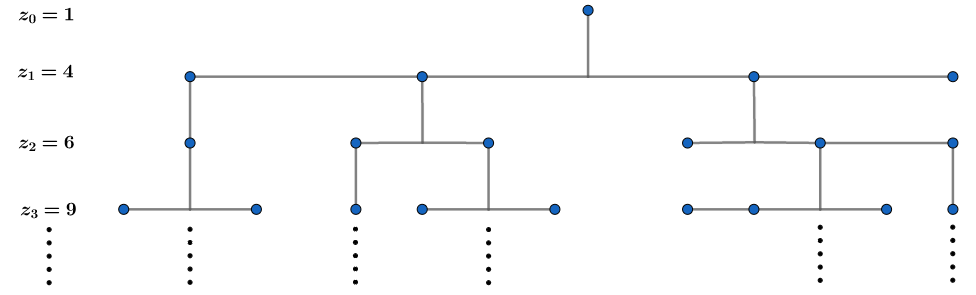
\includegraphics[scale=0.45]{G-WTree.png}
\caption*{\textbf{Arbre de Galton-Watson}}
\centering
\end{figure}
\\
$Z_{0} = 1$\\\\
En les següents generacions, el nombre de fills ve donat per la v.a. $X$.\\\\
$Z_{1} =$ nº de fills del primer individu (generació 0), seguint $X$.\\
$Z_{2} =$ nº de fills dels individus de la generació 1.\\
.\\
.\\
.\\
$Z_{n} =$ nº de descendents en la generació n-èssima.\\\\

\underline{Propietat fonamental}: el nombre de descendents d'un individu és independent del 
nombre de descendents de qualsevol altre individu. \\

\begin{lema}
  Sigui $N$ una variable aleatòria amb imatge en $\setb{1,2,3,\ldots}$.\\
  $X_{1},X_{2},X_{3},\ldots$ variables aleatòries independents (i independents amb $N$), amb 
  $X_{i}\sim X$. Prenem $Y=X_{1}+X_{2}+\ldots +X_{N}$\\
  $\implies G_{Y}(z)=G_{N}(G_{X}(z))$
\end{lema}

\begin{prop}
  $G_{Z_{n+m}}(z) = G_{Z_{n}}(G_{Z_{m}}(z))$. En particular $G_{Z_{n}}(z)=G_{X}\circ \overset{n)}{\ldots} \, \circ G_{X}(z)$
\end{prop}

\begin{obs}
  Podem calcular $\E[Z_{n}]$ i $\V ar[Z_{n}]$ a partir de la seva funció generadora de probabilitat:
  \[
    \E[Z_{n}] = \E[X]^{n}
  \]
  \[
    \V ar[Z_{n}] = 
    \begin{cases}
      n\cdot \V ar[X] \qquad &\text{si } \E[X] = 1 \\\\
      \dfrac{\V ar[X]\cdot (\E[X]^{n}-1)}{\E[X]-1} \quad &\text{si } \E[X]\not =1
    \end{cases}
  \]
\end{obs}

Ara, la pregunta que ens fem és: quan hi haurà extinció?\\
Si fem $A_{n} = \setb{Z_{n} = 0} \implies Extinci\acute o = \bigcup\limits_{n\geq1}A_{n}$\\
$\implies p(Extinci\acute o) = p(\bigcup\limits_{n\geq1}A_{n})$\\\\
$A_{1}\subseteq A_{2}\subseteq A_{3}\subseteq \ldots$\\\\
$
\begin{rcases}
  \text{Extingit a la primera gen}\implies \text{Extingit a la segona gen.} \implies \ldots \\
  \text{Extingit a la segona gen.}\centernot\implies \text{Extingit a la primera} \ldots
\end{rcases} \implies
$
\\\\
$\implies$ Tenim una successió creixent de successos.\\\\
$A_{1}\subseteq A_{2}\subseteq A_{3}\subseteq \ldots$ és creixent $\implies p(Extinci\acute o) = 
\lim\limits_{n\to\infty}p(A_{n}) = \lim\limits_{n\to\infty}p(Z_{n}=0)$\\

\begin{thm}[(Galton)]
  Si $\E[X] = \mu$; $p(X=0) \geq 0$\\
  I sigui $\alpha$ la solució més petita positiva de l'equació $G_{X}(z) = z$ (Aleshores $p(Extinci\acute o) = \alpha$)
  \begin{enumerate}
      \item Si $\mu < 1 \implies \alpha = 1$ \hspace{5.55cm} (\underline{règim subcrític})
      \item Si $\mu = 1 \implies \alpha = 1$ (sempre que $\V ar[X] \not = 0$) \hspace{1cm}(\underline{règim crític})
      \item Si $\mu > 1 \implies 0<\alpha<1$ \hspace{4.85cm} (\underline{règim supercrític})
  \end{enumerate}
\end{thm}

\newpage
\section{Variables Aleatòries Contínues}
\subsection{Mesures de probabilitat absolutament contínues. Funció de densitat}
Sigui $(\Omega, \mathcal{A},p)$ un espai de probabilitat, amb probabilitat induïda en $(\real, \mathcal{B},p_{X})$ (quan prenem la variable aleatòria $X$).

\begin{defi}
  Siguin$\mu_{1},\mu_{2}$ mesures sobre un espai de mesura $(X,\mathcal{A})$, diem que $\mu_{1}$ és \textbf{absolutament contínua} respecte $\mu_{2}$ ($\mu_{1}<<\mu_{2}$) si $\forall A\in \mathcal{A}$,
  \[
    \mu_{2}(A)=0 \implies \mu_{1}(A)=0
  \]
\end{defi}

\begin{defi}
  Una variable aleatòria $X$ és \textbf{absolutament contínua} (o contínua per abreujar), si $p_{X}<<\lambda$ ($\lambda$ és la mesura de Lebesgue).
\end{defi}

\begin{obs}
  Les variables aleatòries discretes \underline{no} són absolutament contínues: \\
  Si $p(X=a)=P_{a}>0$ i prenem $B=\setb{a}$, tenim $\lambda(\setb{a})=0$, però $p_{X}(\setb{a})=P_{a}>0$
\end{obs}

El teorema fonamental que ens permet traduir $p_{X}$ (si $X$ és absolutament contínua) a càlculs usant la mesura $\lambda$, és el següent:

\begin{thm}[(Radon-Nikodym)]
  Sigui $(X,\mathcal{A})$ un espai mesurable i $\mu_{1},\mu_{2}$ mesures sobre $(X,\mathcal{A})$ amb $\mu_{1}<<\mu_{2}$. Aleshores, existeix una funció $f_{\mu_{1}}$, $\mu_{2}$-mesurable tal que
  \[
    \forall A \in \mathcal{A}, \, \mu_{1}(A)=\int_{A}f_{\mu_{1}}d\mu_{2}
  \]
  A més, $f_{\mu_{1}}$ és única $\mu_{2}$-gairebé arreu
\end{thm}

\begin{defi}
  La funció $f_{\mu_{1}}$ és la \textbf{funció de densitat} de la mesura $\mu_{1}$ respecte a $\mu_{2}$. \\
  En el nostre context, $X$ és una variable aleatòria absolutament contínua, i
  \[
    \begin{rcases}
      (\real, \mathcal{B},\underbrace{\lambda}_{\mu_{2}})\\
      (\real, \mathcal{B}, \underbrace{p_{X}}_{\mu_{1}})
    \end{rcases}\underset{\mathclap{X abs. cont.}}{\implies} \, p_{X}<<\lambda\overset{R-N}{\implies} \forall B \in \mathcal{B}, \, \boxed{p_{X}(B)=\int_{B}f_{X}d\lambda}
  \]
\end{defi}

\begin{defi}
  La funció $f_{X}$ s'anomena \textbf{funció de densitat de probabilitat} de $X$.
\end{defi}

\begin{obs}
  En la literatura, s'escriu $f_{\mu_{1}}=\dfrac{d\mu_{1}}{d\mu_{2}}$ (Derivada de Radon-Nikodym).
\end{obs}

\newpage

\begin{prop}
  Si $X$ és una variable aleatòria absolutament contínua, amb funció de densitat de probabilitat $f_{X}(x)$:
  \begin{enumerate}
      \item $f_{X}(x)\geq0$ $\lambda$-gairebé arreu
      \item $F_{X}(x)=\int_{(-\infty,x)}f_{x}d\lambda$; $\qquad \int_{\real}f_{X}d\lambda=1$
      \item $p(X=x)=\int_{\setb{x}}f_{X}d\lambda=0 \, \forall x \in \real$
      \item Si $f_{X}$ és integrable Riemann, $F_{X}(x)=\int_{-\infty}^{x}f_{X}(x)dx$ i $\dfrac{dF_{X}(x)}{dx}=f_{X}(x)$
  \end{enumerate}
\end{prop}

\begin{obs}
  Tota funció mesurable $f(x)$ que compleixi: 
  \[
    \int_{\real}fd\lambda=1, \quad f(x)\geq 0 \qquad \lambda \text{-gairebé arreu.}
  \]
  Aleshores $\exists X$ variable aleatòria absolutament contínua per la qual $f(x)=f_{X}(x)$. \\
  En aquest context, tenim:
  \[
    \E[X]= \int_{\Omega}Xdp = \int_{\real}xdp_{X} \overset{R-N}{=}\int_{\real}x\underbrace{f_{X}(x)d\lambda}_{dp_{X}} \underset{si f_{X} int. R.}{=} \int_{-\infty}^{+\infty}xf_{X}(x)dx
  \]
  En particular,
  \[
    \V ar[X] = \int_{-\infty}^{+\infty}x^{2}f_{X}(x)dx - \bigg( \int_{-\infty}^{+\infty}xf_{X}(x)dx \bigg)^{2}
  \]
\end{obs}

\subsection{Models de variables aleatòries absolutament contínues}

\begin{enumerate}
    \item \underline{Uniforme}: $X \sim U([a,b])$ \quad (Tria un nombre uniformement a l'atzar en l'interval $[a,b]$). \\
    \[
      f_{X}(x)=\frac{1}{b-a}\mathbbm{1}_{[a,b]}(x)
    \]
    \[
      \E[X]=\frac{b+a}{2}
    \]
    \[
      \V ar[X]=\frac{(b-a)^{3}}{12}
    \]
    \item \underline{Exponencial}: $X\sim Exp(\lambda)$ \quad (S'usa per modelar el tipus de vida d'un aparell. És l'anàleg continu de la Poisson).
    \[
      f_{X}(x)=\lambda\cdot e^{-\lambda\cdot x}\cdot \mathbbm{1}_{[0,+\infty)}(x)
    \]
    \[
      \E[X]=\frac{1}{\lambda}
    \]
    \[
      \V ar[X]=\frac{1}{\lambda^{2}}
    \]
    \item \underline{Normal}: $X\sim N(\mu, \sigma^{2})$ \quad ($\mu \in \real, \, \sigma > 0$)
    \[
      f_{X}(x)=\frac{1}{\sqrt{2\pi\sigma^{2}}}\cdot e^{-\frac{(x-\mu)^{2}}{2\sigma^{2}}}
    \]
    \[
      \E[X]=\mu
    \]
    \[
      \V ar[X]=\sigma^{2}
    \]
    \item \underline{Gamma}: $X \sim \Gamma(\lambda, \tau)$
    \[
      f_{X}(x)=\frac{1}{\Gamma(\tau)}\cdot \lambda^{\tau}\cdot x^{\tau -1}\cdot e^{-\lambda x}\cdot \mathbbm{1}_{[0,+\infty)}(x)
    \]
    \[
      \E[X]=\frac{\tau}{\lambda}
    \]
    \[
      \V ar[X]=\frac{\tau}{\lambda^{2}}
    \]
    \item \underline{Weibull}: $X\sim Weib(\alpha, \beta)$
    \[
      f_{X}(x)=\alpha\cdot \beta \cdot x^{\beta-1}\cdot e^{-\alpha\cdot x^{b}}\cdot \mathbbm{1}_{[0,+\infty)}(x)
    \]
    \[
      \E[X]=\alpha^{-\frac{1}{\beta}}\cdot \Gamma(1+\frac{1}{\beta})
    \]
    \[
      \V ar[X]=\alpha^{-\frac{2}{\beta}}(\Gamma(1+\frac{2}{\beta})-\Gamma^{2}(1+\frac{1}{\beta}))
    \]
    \item \underline{Beta}: $X\sim \beta(a,b)$
    \[
      f_{X}(x)=\frac{\Gamma(a+b)}{\Gamma(a)\cdot \Gamma(b)}\cdot x^{a-1}\cdot (1-x)^{b-1}\cdot \mathbbm{1}_{[0,1]}(x)
    \]
    \[
      \E[X]=\frac{a}{a+b}
    \]
    \[
      \V ar[X]=\frac{a\cdot b}{(a+b)^{2}\cdot (a+b+1)}
    \]
    \item \underline{Cauchy}: $X\sim Cauchy$
    \[
      f_{X}(x)=\frac{1}{\pi\cdot (1+x^{2})} \quad (x \geq 0)
    \]
     \quad Cap dels $\E[X^{k}]$ és finit.
\end{enumerate}

\subsection{Distribucions conjuntes i marginals. Independència i distribucions condicionades}

Ara farem el mateix que per una variable en el cas de tenir vectors de variables aleatòries.\\
Ho farem per vectors $(X_{1},X_{2})$, però és fàcilment generalitzable a vectors de dimensió $> 2$. \\
Sigui $(X,Y)$ un vector de variables aleatòries. $(X,Y)$ indueix $p_{(X,Y)}$ mesura de probabilitat en $\real^{2}$.

\begin{defi}
  $(X,Y)$ és un \textbf{vector absolutament continu} si $p_{(X,Y)}<<\lambda_{\real^{2}}$. \\
  Per $Radon-Nikodym$, $(X,Y)$ té una \textbf{funció de densitat}:
  \[
    B\in\mathcal{B}_{\real^{2}}, \, p_{(X,Y)}(B)=\iint_{B}f_{(X,Y)}d\lambda_{\real^{2}}
  \]
\end{defi}

\begin{defi}
  $f_{X,Y}(x,y)$ és la \textbf{funció de densitat conjunta} de $X$ i $Y$.\\
  Si ara $B=(a_{1},a_{2})\times(b_{1},b_{2})$ i $f_{(X,Y)}(x,y)$ és integrable Riemann, 
  \[
    p_{(X,Y)}(B)=\iint_{B}f_{(X,Y)}\,d\lambda_{\real^{2}}=\int_{a_{1}}^{a_{2}}\int_{b_{1}}^{b_{2}}f_{(X,Y)}(x,y)\,dy\,dx
  \]
\end{defi}

A partir de $f_{(X,Y)}(x,y)$ podem extreure la funció de densitat de $X$ i de $Y$ integrant:

\begin{defi}
  Donat un vector de variables aleatòries $(X,Y)$ amb funció de densitat conjunta $f_{(X,Y)}(x,y)$, les \textbf{funcions de densitat marginals} són:
  \[
    f_{X}(x) = \int_{-\infty}^{+\infty}f_{(X,Y)}(x,y) \, dy
  \]
  \[
    f_{Y}(y) = \int_{-\infty}^{+\infty}f_{(X,Y)}(x,y) \, dx
  \]
\end{defi}

A partir de la funció de densitat conjunta podem definir la \textbf{funció de distribució}: 
\[
  F_{(X,Y)}(x,y) = P(X \leq x, Y \leq y) \underset{int. Riem.}{=} \int_{-\infty}^{x}\int_{-\infty}^{y} f_{(X,Y)}(x,y) \, dy \, dx
\]

\begin{obs}
  Si $f_{X,Y}(x,y)$ és integrable Riemann $\implies F_{(X,Y)}(x,y)$ és $\mathcal{C}^{2}(\real^{2})$ i
  \[
    \frac{\partial^{2}F_{(X,Y)}}{\partial x \partial y}(x,y) = \frac{\partial^{2}F_{(X,Y)}}{\partial y \partial x}(x,y) = f_{(X,Y)}(x,y)
  \]
\end{obs}

\begin{obs}
  Si $g:\real^{2} \to \real$ és una funció mesurable, $g(X,Y)$ és una variable aleatòria i es compleix:
  \[
    \E[g(X,Y)] = \iint_{\real^{2}} g(x,y)\cdot f_{(X,Y)}(x,y) \, dx \, dy
  \]
\end{obs}


\subsubsection{Independència}

Si $(X,Y)$ és un vector aleatori i $X$, $Y$ són independents, aleshores $F_{X,Y}(x,y) = F_{X}(x)\cdot F_{Y}(y)$. Ara si $F_{(X,Y)}$ és $\mathcal{C}^{2}$ i les $F_{X}$, $F_{Y}$ són derivables (això sempre passa en el cas absolutament continuu), llavors

\[
  f_{(X,Y)}(x,y) = \frac{\partial^{2}F_{(X,Y)}}{\partial x \partial y} = \frac{\partial F_{X}}{\partial x}\cdot \frac{\partial F_{Y}}{\partial y} = f_{X}(x) \cdot f_{Y}(y)
\]

Per tant, $X$ i $Y$ variables aleatòries absolutament contínues són independents sii
\[
  f_{(X,Y)}(x,y) = f_{X}(x)\cdot f_{Y}(y)
\]

\underline{Notació}: si $(X,Y)$ és un vector aleatori, 
\[
  \E[(X,Y)] = (\E[X], \E[Y])
\]

\[
  \V ar[(X,Y)] = 
  \begin{pmatrix}
    \V ar[X]  &  Cov(X,Y) \\
    Cov(X,Y)  &  \V ar[Y]
  \end{pmatrix}
  \underset{Si X,\, Y ind}{=}
  \begin{pmatrix}
    \V ar[X]  &  0 \\
    0         &  \V ar[Y]
  \end{pmatrix}
\]

\subsubsection{Distribucions condicionades}

Siguin $X$, $Y$ variables aleatòries absolutament contínues, amb funció de densitat conjunta $f_{(X,Y)}(x,y)$ i marginals $f_{X}(x)$, $f_{Y}(y)$. Sigui $x$ tal que $f_{X}(x) > 0$.

\begin{defi}
  La veriable aleatòria $Y \mid X = x$ és una variable aleatòria que té com a funció de distribució:
  \[
    F_{Y\mid X}(y,x) = \frac{1}{f_{X}(x)} \cdot \int_{-\infty}^{y}f_{(X,Y)}(x,u) \, du
  \]
  Si $f_{(X,Y)}(x,y)$ és integrable respecte a y, aleshores, $F_{Y \mid X}(y,x)$ és derivable respecte a $y$, i es compleix:
  \[
    f_{Y\mid X}(y,x) = \frac{\partial F_{Y\mid X}(y,x)}{\partial y} = \frac{f_{(X,Y)(x,y)}}{f_{X}(x)}
  \]
\end{defi}

\subsubsection{Esperança condicionada}

En les condicions d'abans, definim:
\[
  \E[Y\mid X=x] = \int_{-\infty}^{+\infty}u\cdot f_{Y\mid X}(u,x)\, du = \psi(x) \implies \E[Y\mid X] = \psi(X)
\]

Totes les propietats que vam veure en el cas discret per l'esperança condicionada s'apliquen aquí de la mateixa manera. En particular:

\begin{prop}
  \[
    \E\big[\,\E[Y\mid X]\,\big] = \E[Y] \qquad \text{(si $(X,Y)$ és abs. cont.)}
  \]
\end{prop}

\subsection{Funcions de v.a. absolutament contínues i aplicacions}

Sigui $\overrightarrow{X} = (X_{1}, \ldots , X_{n})$ un vector aleatori absolutament 
continuu i $G:\real^{n} \to \real^{n}$ una funció bijectiva. \\

Com relacionem $f_{(X_{1},\ldots, X_{n})}(x_{1},\ldots,x_{n})$ amb $f_{(Y_{1},\ldots, Y_{n})}(y_{1},\ldots,y_{n})$?

\subsubsection{Cas univariat}
Sigui $X$ una variable aleatòria absolutament contínua amb funció de densitat $f_{X}(x)$. Sigui $g:\real \to \real$ una funció bijectiva, derivable i estrictament creixent. Considerem ara $g(X) = Y$ (i $\inv{g} = h$). Aleshores,

\[f_{Y}(u) \text{ i } f_{X}(h(u))\cdot h'(u) \text{ són iguals } \lambda-gaireb\acute{e} \, per \, tot\]

\begin{obs}
  Si $g$ no és bijectiva o no és estrictament creixent, en general l'anàlisi és més complicat.
\end{obs}

\subsubsection{Cas multivariat}
$G(\overrightarrow{X}) = \overrightarrow{Y}$ on $G$ és bijectiva i $\mathcal{C}^{1}(\real^{n})$, aleshores, de manera similar al cas anterior, tenim:
\[
  f_{(Y_{1},\ldots,Y_{n})}(y_{1},\ldots,y_{n}) = f_{(X_{1},\ldots,X_{n})}(\inv{G}(y_{1},\ldots,y_{n}))\cdot \abs{Jac\,\inv{G}(y_{1},\ldots,y_{n})}
\]

\subsection{Distribució normal, multivariant i distribucions associades}

Ja vam veure que la distribució normal ve donada per la seva esperança i la seva variància: 
\[
  X \sim N(\mu, \sigma^{2})
\]
\[
  f_{X}(x) = \frac{1}{\sqrt{2\pi\sigma^{2}}}\cdot e^{\frac{-1}{2\sigma}\cdot(x-\mu)^{2}}
\]

La suma de normals independents és normal.

\begin{thm}[(Moivre-Laplace)]
  Sigui $X\sim Bin(n,p)$. Aleshores 
  \[
    p\Bigg(a \leq \frac{X-np}{\sqrt{np(1-p)}}\leq b\Bigg)\xrightarrow[n\to\infty]{} \int_{b}^{a} \frac{1}{\sqrt{2\pi}}\cdot e^{-\frac{x^{2}}{2}}\, dx
  \]
\end{thm}

\newpage

\subsubsection{Distribucions associades a la normal}
\begin{itemize}
    \item $X_{i}\sim N(0,1)$; $X_{1}, \, X_{2},\ldots$ independents. 
    \[
      X_{1}^{2}+X_{2}^{2}+\ldots+X_{n}^{2}=\chi_{n}^{2} \quad \equiv \textbf{Chi quadrat} \text{ (amb n graus de llibertat})
    \]
    \item Si tenim $\chi_{d_{1}}^{2}$ i $\chi_{d_{2}}^{2}$, aleshores
    \[
      \frac{^{\chi_{d_{1}}^{2}} / _{d_{1}}}{^{\chi_{d_{2}}^{2}} / _{d_{2}}} \equiv \textbf{F-Fisher-Snedecor} \text{ (amb paràmetres $d_{1}$ i $d_{2}$)}
    \]
    \item $X\sim N(0,1)$, $\chi_{k}^{2}$ independent de $X$.
    \[
      \frac{X}{\sqrt{^{\chi_{k}^{2}} / _k}} \equiv \textbf{t - de Student} \text{ (amb $k$ graus de llibertat)}
    \]
\end{itemize}

\subsubsection{Normal multivariant}

\begin{defi}
  Sigui $\overrightarrow{X}=(X_{1},\ldots,X_{n})$ un vector aleatori, direm que $\overrightarrow{X}$ és un \textbf{vector de variables aleatòries normal multivariant} si la seva funció de densitat conjunta és:
  \[
    f_{\overrightarrow{X}}(x_{1},\ldots,x_{n}) = f_{\overrightarrow{X}}(\overrightarrow{x}) = \frac{1}{\sqrt{(2\pi)^{n}\cdot \abs{det(\Sigma)}}}\cdot e^{-\frac{1}{2}(\overrightarrow{x}-\overrightarrow{\mu})^{T}\cdot \inv{\Sigma} \cdot (\overrightarrow{x}-\overrightarrow{\mu})}
  \]
  on
  \begin{itemize}
      \item  $\overrightarrow{\mu}$ és un vector de $\real^{n}$ (vector d'esperances)
      \item $\Sigma$ és una matriu $n\times n$ simètrica i definida positiva (matriu de covariàncies)
  \end{itemize}
  \[
    \overrightarrow{\mu} = \E[\overrightarrow{x}]
  \]
  \[
    \Sigma = \Big( Cov(x_{i},x_{j})\Big)_{i,j}
  \]
\end{defi}

\underline{Cas particular}: Si $\Sigma = Id$, $\overrightarrow{\mu} = \overrightarrow{0}$, aleshores escriurem $\overrightarrow{X}=\overrightarrow{U}$ i es compleix que 
\[
f_{\overrightarrow{U}}(\overrightarrow{x}) = \frac{1}{\sqrt{(2\pi)^{n}}}\cdot e^{-\frac{1}{2}\cdot(\overrightarrow{x}-\overrightarrow{\mu})^{T}\cdot  (\overrightarrow{x}-\overrightarrow{\mu})} = \frac{1}{\sqrt{(2\pi)^{n}}}\cdot e^{-\frac{1}{2}\cdot\sum\limits_{i=1}^{n}x_{i}^{2}} = \prod_{i=1}^{n} f_{x_{i}}(x_{i})
\]
Per tant, les marginals són normals univariades i independents. \\

Ara veurem que tot vector normal multivariant s'obté de fet com una transformació lineal de $\overrightarrow{U}$.

\begin{thm}
  $\overrightarrow{X}=(X_{1},\ldots,X_{n})$ segueix una llei normal multivariant $\iff \overrightarrow{X} = A\cdot\overrightarrow{X} + \overrightarrow{b}$ on $A$ és una matriu \underline{no} singular ($\Sigma = A^{T}\cdot diag \cdot A$).
\end{thm}

\begin{thm}
  Sigui $\overrightarrow{X}\sim N(\overrightarrow{\mu}, \Sigma)$ de dimensió $n$, i $M$ una matriu $m\times n$ de rang màxim ($m\leq n$). Aleshores $M\cdot\overrightarrow{X}$ és un vector de variables aleatòries normal multivariant $N(M\cdot\overrightarrow{\mu}, M\cdot\Sigma\cdot M^{T})$.
\end{thm}
\-\\
En el cas de $m = 1$ tenim el següent corol·lari:

\begin{col}
  Si $a_{1},\ldots,a_{n}$ són nombres tals que $\sum a_{i}^2 > 0$ (la matriu $(a_{1},\ldots,a_{n})$ té rang 1) i $\overrightarrow{X}\sim N(\overrightarrow{\mu}, \Sigma)$, $\overrightarrow{X} = (X_{1},\ldots,X_{n})$
  \[
    M\overrightarrow{X} = \sum_{i=1}^{n} a_{i}x_{i} \sim N\bigg(\sum_{i=1}^{n} a_{i}\mu_{i}, \sum a_{i}^{2}\sigma_{i}^{2} + 2\sum_{i<j}a_{i}a_{j}\sigma_{ij}\bigg) \quad \text{ on } 
    \begin{cases}
      \overrightarrow{\mu} = (\mu_{1},\ldots,\mu) \\
      \sigma_{i}^{2} = \V ar[X_{i}] \\
      \sigma_{ij} = Cov(X_{i}, X_{j})
    \end{cases}
  \]
\end{col}

\-\\
Seguidament veurem els estimadors i el teorema de Fisher:

\begin{defi}
  Siguin $X_{1}, X_{2}, \ldots, X_{n}$ variables aleatòries idènticament distribuïdes. L'\textbf{esperança mostral} i la \textbf{variància mostral} són: \\
  \[
    \overline{X} = \frac{X_{1}+\ldots+X_{n}}{n}
  \]
  \[
    S^{2} = \frac{1}{n-1}\cdot\sum_{i=1}^{n}(x_{i} - \overline{X})^{2}
  \]
  \-\\
  En particular, $\E[\overline{X}] = \E[X_{1}]$, $\V ar[\overline{X}] = \frac{\V ar[X_{1}]}{n}$ i $\E[S^{2}] = \V ar[X_{1}]$ \\
  
\end{defi}

Si, a més, $X_{1},\ldots,X_{n}$ són $N(\mu,\sigma^{2})$, tenim el següent teorema:

\begin{thm}[(Fisher)]
  Si $X_{1},\ldots, X_{n}$ són independents i $N(\mu, \sigma^{2})$, aleshores $\overline{X}$ i $S^{2}$ són independents. \\ 
  A més, $\overline{X} \sim N(\mu, \frac{\sigma^{2}}{n})$ i $S^{2} \sim \chi_{n-1}^{2}$
\end{thm}

\newpage
\section{Funcions característiques i famílies exponencials}

\subsection{Funció generadora de moments i funció característica}

\begin{defi}
  Sigui $(\Omega, \mathcal{A}, p)$ un espai de probabilitat i $X$ una variable aleatòria, la \textbf{funció generadora de moments} de $X$ és $M_{X}(s)$, definida per:
  \[
    M_{X}(s) = \E[e^{sX}] \quad \text{ on s $\in \cx \quad$ (No té per què estar definida)}
  \]
\end{defi}

\begin{properties}\-
  \begin{enumerate}
      \item $M_{X}(0) = 1$
      \item Si $\E[X^{k}] < \infty \,\, \forall k \geq 1\text{, aleshores }\E[X^{k}]=M_{X}^{(k)}(0)$
      \item Si $Y=aX+b$,
      \[
        M_{Y}(s) = \E[e^{s\cdot(aX+b)}] = e^{sb}\E[e^{saX}] = e^{sb}\cdot M_{X}(as)
      \]
      \item Si $X,Y$ són indep. $\implies M_{X+Y}(s) = \E[e^{s\cdot(X+Y)}] = \E[e^{sX}]\cdot\E[e^{sY}] = M_{X}(s)\cdot M_{Y}(s)$
  \end{enumerate}
\end{properties}
\-\\
Aquesta definició particularitza en el cas discret i en el cas continuu de la següent manera:
\begin{itemize}
    \item Cas discret: $\E[e^{sX}] = \sum\limits_{x\in Im(X)}e^{sx}p(X=x)$
    \item Cas continuu: $\E[e^{sx}] = \int_{\real}e^{sx}f_{X}(x) \, dx$
\end{itemize}

\begin{example}
  \begin{itemize}
  \item[]
      \item $X \sim Ber(p) \implies M_{X}(s) = e^{s\cdot0}\cdot(1-p) + e^{s\cdot1}\cdot p = p\cdot e^{s} + (1-p)$ \\\\
      $M_{X}(s)$ és una funció entera $\implies$ podem calcular tots els moments: $\E[X^{k}] = p$ \\
      \item Si $Y \sim Bin(N,p) \implies Y=X_{1}+\ldots+X_{N} \quad \text{on } X_{i}\sim Ber(p), \, \setb{X_{i}}_{i=1}^{N} \text{ independents}$
      \[
        M_{Y}(s) = (p\cdot e^{s} + (1-p))^{N}
      \]
      \item $X\sim Exp(\lambda) \quad (\lambda > 0)$
      \[
        M_{X}(s) = \int_{\real}e^{sx}\cdot\lambda e^{-\lambda x} \, dx = \lambda\int_{-\infty}^{+\infty} e^{(s-\lambda)x} \, dx = \lambda\cdot\frac{e^{(s-\lambda)x}}{s-\lambda}\bigg|_{-\infty}^{+\infty}
      \]
      (No està definida per alguns valors de $s$)
      \item $X \sim Cauchy. \, X$ té funció de densitat $\dfrac{1}{\pi(1+x^{2})}$
      \[
        \E[e^{sX}] = \int_{\real}\frac{e^{sx}}{\pi(1+x^{2})}\, dx \quad \text{(No té sentit si $Re(s)>0$)}
      \]
  \end{itemize}
  
\end{example}

\newpage
  
Estem veient que la funció generadora de moments no convergeix en la majoria de casos. Això és degut a que $s\in\cx$. \\
Per a solucionar aquest problema, prenem $s=it$ ($t\in\real$).

\begin{defi}
  La funció $\E[e^{itX}] = M_{X}(it) = \Phi_{X}(t)$ és la \textbf{funció característica} de X.
\end{defi}

\begin{obs}
  Totes les propietats de la funció generadora de moments es compleixen per les funcions característiques:
  \begin{enumerate}
      \item  $\Phi_{X}(0) = 1$
      \item $\E[X^{k}] = M_{X}^{(k)}(0) = \dfrac{d^{k}}{ds^{k}}M_{X}(s)\bigg|_{s=0} = \dfrac{1}{(i)^{k}}\cdot \Phi_{X}^{(k)}(0)$
      \item $Y = aX+b \implies \Phi_{Y}(t) = e^{ibt}\cdot \Phi_{X}(at)$
      \item $X,Y$ independents $\implies \Phi_{X+Y}(t)=\Phi_{X}(t)\cdot\Phi_{Y}(t)$
  \end{enumerate}
\end{obs}

\begin{example}
  \begin{itemize}
      \item[]
      \item $X\sim Exp(\lambda) \quad (\text{amb } \lambda > 0)$. Té funció de densitat $f_{X}(x) = \lambda e^{-\lambda x}\cdot \mathbbm{1}_{[0, \infty)}(x)$
      \[
        \Phi_{X}(t) = \int_{0}^{\infty}e^{itx}\cdot\lambda e^{-\lambda x} \, dx = \lambda\int_{0}^{\infty}e^{(it-\lambda)x} \, dx = \lambda\frac{e^{(it-\lambda)x}}{it-\lambda}\bigg|_{0}^{\infty} = \frac{-\lambda}{it-\lambda}
      \]
      (Està definida per tot valor de t)
      \item $X\sim Cauchy$
      \[
        \Phi_{X}(t) = \int_{-\infty}^{+\infty}\frac{e^{itx}}{\pi(1+x^{2})} \, dx = e^{-\abs{t}}
      \]
      S'observa que la variable aleatòria $Cauchy$ \underline{no} té moment, però si que té funció característica (No es pot derivar $\Phi_{X}(t)$ en $t=0$)
      \item $X\sim N(0,1)$ : $\Phi_{X}(t) = e^{\frac{-t^{2}}{2}}$ \\\\
      Com a conseqüència, si $X\sim N(\mu, \sigma^{2})$, aleshores $X=\sigma Y + \mu$ (on $Y\sim N(0,1)$)
      \[
        \implies \Phi_{X}(t) = e^{i\mu t - \frac{1}{2}\sigma^{2}t^{2}}
      \]
      
      \item $X\sim Geom(p)$: $\Phi_{X}(t) = \dfrac{p}{e^{it}-(1-p)}$
      \item $X\sim Pois(\lambda)$: $\Phi_{X}(t) = e^{\lambda(e^{it}-1)}$
      \item $X\sim U(0,1)$: $\Phi_{X}(t) = \dfrac{e^{it}-1}{it} \quad$ (Té una singularitat evitable en t=0)
  \end{itemize}
\end{example}

\subsubsection{Propietats generals de les funcions característiques}
\begin{prop}
  Sigui $X$ una variable aleatòria amb funció característica $\Phi_{X}(t)$. Aleshores:
  \begin{enumerate}
      \item $\Phi_{X}(0)=1$ i $\abs{\Phi_{X}(t)}\leq 1 \, \forall t\in\real$
      \item $\Phi_{X}(t)$ és uniformement contínua en $\real$.
      \item $\forall t_{1},\ldots,t_{n} \in \real, \forall z_{1},\ldots,z_{n}\in\cx$, $\sum\limits_{j,k}\Phi_{X}(t_{j}-t_{k})z_{j}\cdot \overline{z}_{k}\geq0$
  \end{enumerate}
\end{prop}

\begin{thm}[(d'inversió)]
  Sigui $X$ una variable aleatòria que indueix una probabilitat $p_{X}$ sobre $\real$ i funció característica $\Phi_{X}(t)$. Aleshores $\forall a,b\in \real \, (a<b)$,
  \[
    \underbrace{p_{X}\big((a,b)\big)}_{p(a<X<b)} + \frac{1}{2}\big(p_{X}(\setb{a})+p_{X}(\setb{b}) \big) = \lim_{T\to+\infty}\frac{1}{2\pi}\int_{-T}^{T}\frac{e^{-ita}-e^{-itb}}{it}\cdot\Phi_{X}(t) \, dt
  \]
\end{thm}

\begin{lema} \-\\
  Donada una variable aleatòria $X$, el nombre de discontinuïtats de $F_{X}(x)$ és un conjunt numerable.
\end{lema}

\begin{col}
  $\Phi_{X}(t)$ caracteritza completament $X$.
\end{col}

\subsection{Famílies exponencials}

Ara veurem que podem tractar de manera molt general famílies de variables aleatòries usant la noció de família exponencial.

\begin{defi}
  Una família de variables aleatòries és \textbf{exponencial} amb paràmetres $\overrightarrow{\theta} = (\theta_{1},\ldots,\theta_{n})$ si la funció de probabilitat (cas discret) o la funció de densitat (cas continuu) té la forma:
  \[
    p(x\mid \overrightarrow{\theta}) = f(x,\overrightarrow{\theta}) = g(x)\cdot \exp\Big(\sum_{i=1}^{n}\theta_{i}t_{i}(x)-C(\overrightarrow{\theta})\Big) \quad \text{ (on $\setb{t_{i}(x)}_{i=1}^{n}$ són funcions l.i.)}
  \]
  La família es diu \textbf{natural} si $\exists k$ tal que $t_{k}(x)=x$.
\end{defi}

\begin{example}
  \begin{enumerate}
  \item[]
      \item $X\sim Ber(p)$
      \[
        p(x\mid p) = p^{x}(1-p)^{1-x} = \exp\Big(x\cdot \log(p) + (1-x)\cdot \log(1-p)\Big), \quad x\in\setb{0,1}
      \]
      Agafem l'exponent:
      \[
        x\cdot \log(p) + (1-x)\cdot \log(1-p) = x\Big(\log(p) - \log(1-p)\Big) = x\bigg(\underbrace{\log\Big(\frac{p}{1-p}\Big)}_{\theta} \bigg) + \log(1-p)
      \]
      Si fem $\theta = \log\Big(\dfrac{p}{1-p}\Big) \implies e^{\theta} = \dfrac{p}{1-p} \implies e^{\theta} - pe^{\theta} = p \implies p = \dfrac{e^{\theta}}{1+e^{\theta}}$
      \[
        \implies \log(1-p) = \log\bigg(1-\frac{e^{\theta}}{1+e^{\theta}}\bigg) = -\log(1+e^{\theta})
      \]
      Per tant, 
      \[
        p(x\mid \theta) = \exp\Big(\underset{\substack{\downarrow \\ t_{1}(x)}}{x}\cdot\theta - \underbrace{\log(1+e^{\theta})}_{C(\theta)}\Big) \qquad \bigg(\theta = \log\frac{p}{1-p}\bigg)
      \]
      és família exponencial natural.
      \item $X\sim Bin(N,p)$
      \[
        p(x\mid N,p) = \binom{N}{x}\cdot p^{x}(1-p)^{N-x} \quad x \in \setb{0,1,\ldots,N}
      \]
      $N$ no pot ser un paràmetre! $\implies N$ ha de ser fix. \\\\
      En aquesta situació: \\\\
      $
        p(x\mid p) = \underbrace{\binom{N}{x}}_{g(x)} p^{x}(1-p)^{N-x} = g_{N}(x)\cdot \exp\Big(x\cdot \log(p) + (N-x)\cdot \log(1-p)\Big) = \\=g_{N}(x)\cdot \exp\Big(x\cdot \log(\frac{p}{1-p}) + N\cdot \log(1-p)\Big) \underset{\theta = \log\frac{p}{1-p}}{=}
        g_{N}(x)\cdot \exp\big(x\cdot\theta - N\cdot \underbrace{\log(1+e^{\theta})}_{C(\theta)}\big)
      $
      \item $X\sim N(\mu, \sigma^{2})$
      \[
        p(x\mid \mu, \theta) = \frac{1}{\sqrt{2\pi\sigma^{2}}}\cdot \exp\bigg(\frac{-(x-\mu)^{2}}{2\sigma^{2}}\bigg) = \frac{1}{\sqrt{2\pi}}\cdot \exp\bigg(\frac{-(x-\mu)^{2}}{2\sigma^{2}}-\log(\sigma)\bigg)
      \]
      Desenvolupem l'exponencial:
      \[
      \begin{split}
          \frac{-(x-\mu)^{2}}{2\sigma^{2}}-\log(\sigma) &= \frac{-x^{2}}{2\sigma^{2}}+\frac{2x\mu}{2\sigma^{2}}-\frac{-\mu^{2}}{2\sigma^{2}}-\log(\sigma) = \\
          &= \frac{-x^{2}}{2\sigma^{2}} + \frac{\mu}{\sigma^{2}}x - \Big(\frac{\mu^{2}}{2\sigma^{2}}+\log(\sigma)\Big)= \\
          & = \underbrace{\frac{\mu}{\sigma^{2}}}_{\theta_{1}}x \underbrace{-\frac{1}{2\sigma^{2}}}_{\theta_{2}}x^{2} - \Big(\frac{\mu^{2}}{2\sigma^{2}}+\log(\sigma)\Big)= \\
          &= \theta_{1}\cdot\underset{\substack{\downarrow \\ t_{1}(x)}}{x} + \theta_{2}\cdot\underset{\substack{\downarrow \\ t_{2}(x)}}{x^{2}} - \bigg(\underbrace{\frac{-\theta_{1}^{2}}{2\theta_{2}}+\frac{1}{2}\cdot \log\Big(\frac{-1}{2\theta_{2}}\Big)}_{C(\theta_{1},\theta_{2})}\bigg)
      \end{split}
      \]
  \end{enumerate}
\end{example}

\newpage
Estudiant la fórmula $p(x\mid \overrightarrow{\theta})$ directament, podem trobar resultats genèrics de manera senzilla.

\begin{prop}
  $\E[t_{i}(Z)] = \dfrac{\partial}{\partial \theta_{i}}C(\overrightarrow{\theta})$
\end{prop}

\begin{prop}
  Si $X$ pertany a una família exponencial natural amb $t_{1}(x) = x$, aleshores:
  \[
    \Phi_{X}(t) = e^{C(\theta_{1}+it, \theta_{2},\ldots,\theta_{r})-C(\overrightarrow{\theta})}
  \]
\end{prop}

\newpage
\section{Convergència de variables aleatòries}

\subsection{Modes de convergència i equivalències}

Sigui $\{X_n\}_{n\geq1}$ una seqüència de variables aleatòries. Volem donar sentit a la noció de 
convergència de $\{X_n\}_{n\geq1}$ cap a una variable aleatòria $X$ donada.\\
Veurem que això ho podem fer de diverses maneres.

\begin{defi}
  $\{X_n\}_{n\geq1}$ \textbf{convergeix quasi-segurament} cap a $X$, i ho  escriurem $X_n 
  \overset{qs}{\longrightarrow} X$ si
  \[
    p\Big(\underbrace{\setb{\omega \in \Omega : X_n(\omega)\underset{n}{\longrightarrow}X(\omega)}}_{A}\Big) = 1
  \]
  La definició té sentit perquè $A$ és un succés. Vegem-ho:
  \[
    A_n(m) = \setb{\omega \in \Omega : \abs{X_n(\omega) - X(\omega)} < \frac{1}{m}} \text{ és un succés.}
  \]
  \[
    \implies A(m) = \liminf_n A_n(m) = \setb{\omega \in \Omega : \omega \in A_n(m) \quad 
    \forall n \geq n_0(\omega)} \text{ (és un succés)}
  \]
  Finalment,
  \[
    A = \bigcap_{m\geq1}A(m) = \setb{\omega\in\Omega : \forall m \, \exists n_0(\omega) 
    \text{ tal que } \abs{X_n(\omega) - X(\omega)} < \frac{1}{m} \text{ si } n \geq n_0(\omega)} \text{ és un succés.}
  \]
\end{defi}

\begin{defi}
  Direm que $\setb{X_n}_{n\geq1}$ \textbf{convergeix en mitjana d'ordre r} cap a $X$ 
  ($r \geq 1$) i ho escriurem $X_n \overset{r}{\longrightarrow} X$ si
  \[
    \E\left[\abs{X_n - X}^r\right] \underset{n}{\longrightarrow} 0
  \]
\end{defi}

\begin{defi}
  Direm que $\setb{X_n}_{n\geq1}$ \textbf{convergeix en probabilitat} cap a $X$ i ho escriurem 
  $X_n \overset{p}{\longrightarrow} X$ si $\forall \epsilon > 0$
  \[
    p\left(\abs{X_n - X} > \epsilon \right) \underset{n}{\longrightarrow} 0
  \]
\end{defi}

\begin{defi}
  Direm que $\setb{X_n}_{n\geq1}$ \textbf{convergeix en distribució} cap a $X$ i ho escriurem 
  $X_n \overset{d}{\longrightarrow} X$ si
  \[
    F_{X_n}(x) \underset{n}{\longrightarrow} F(x) \text{ en els punts de continuïtat de F(x)}
  \]
\end{defi}

\begin{obs}
  Ens cal que $x$ sigui un punt de continuïtat de $F$ per a que famílies de variables aleatòries 
  convergeixin de manera natural en distribució.
\end{obs}

\newpage

\begin{example}
  Sigui $X$ una variable aleatòria fixada, $X_n = X + \dfrac{1}{n}$. Aleshores volem que 
  $X_n \overset{d}{\longrightarrow} X$. Si això passa, 
  \[
    F_{X_n}(x) = p(X_n \leq x) = p(X \leq x -\frac{1}{n}) \underset{n\to \infty}{\longrightarrow}p(X<x) = F_X(x^-) 
    \quad \text{(límit per l'esquerra)}
  \]
  $\implies$ per tal que $F_X(x)$ sigui $F_X(x^-)$ ens cal suposar que $x$ és un punt de continuïtat de $F_X$.
\end{example}
\-\\\\
El que veurem ara  són implicacions entre els diversos modes de convergència. \\
També veurem que les implicacions contraries mai seran certes.

\subsubsection{Diagrama modes de convergència}

\begin{tikzcd}[arrows=Rightarrow]
X_n \overset{qs}{\longrightarrow} X \arrow[rr, "\text{IV}"] & & X_n \overset{p}{\longrightarrow} X  
\arrow[r, "\text{I}"] & X_n \overset{d}{\longrightarrow} X\\
X_n \overset{r}{\longrightarrow} X \arrow[r, "r>s\geq 1"', "\text{III}"]  & X_n \overset{s}{\longrightarrow} 
X \arrow[ur, "\text{II}"']
\end{tikzcd}

\begin{prop}[(I)]
  $X_n \overset{p}{\to} X \implies X_n \overset{d}{\to} X$, i el recíproc \underline{no} és cert. \\\\
  
  Vegem un contraexemple de que el recíproc no és cert: \\
  
  $X \sim Ber(\dfrac{1}{2})$, $X_n = X$, $Y = 1-X$ (En particular, $Y\sim Ber(\dfrac{1}{2})$). \\
  
  És clar que $X_n \overset{d}{\to} Y$, ja que $X_n \overset{d}{\to} X$ i $X$ i $Y$ tenen la mateixa 
  funció de distribució.
  
  Per altra banda, $\abs{X_n - Y} = 1$ (ja que si una val $1$, l'altra val $0$)
  $$\implies p(\abs{X_n-Y} > \varepsilon) = 1 \quad \text{ si } \varepsilon \text{ és prou petit!!}$$
\end{prop}

\begin{prop}[(II)]
  $X_n \overset{1}{\to} X \implies X_n \overset{p}{\to} X$, i el recíproc \underline{no} és cert. \\\\
  
  Vegem un contraexemple del recíproc: \\
  
  \[
    X_n = \begin{cases}
      n^3 &\text{ amb probabilitat } \frac{1}{n^2} \\
      0   &\text{ amb probabilitat } 1 - \frac{1}{n^2}
    \end{cases}
  \]
  \-\\\\
  
  
  El candidat a límit és $X=0$:
  
  \[ 
    \forall \varepsilon > 0, \, p(\abs{X_n - X} > \varepsilon) = p(\abs{X_n} > \varepsilon) = 
    \frac{1}{n^2} \underset{n\to \infty}{\longrightarrow} 0
  \]
  Amb això, $X_n \overset{p}{\to} 0 = X$. Ara bé,
  \[
    \E\left[\abs{X_n - X}\right] = \E\left[\abs{X_n}\right] = n^3 \cdot \frac{1}{n^2} = 
    n \underset{n \to \infty}{\longrightarrow} \infty \implies X_n \not\overset{1}{\to} 0
  \]
\end{prop}

\begin{prop}[(III)]
  Si $r\geq s \geq 1$ i $ X_n \overset{r}{\to} X \implies X_n \overset{s}{\to} X$.\\\\
  
  El recíproc \underline{no} és cert:
  
  \[
    X_n = \begin{cases}
      n &\text{ amb probabilitat } n^{\frac{-(r+s)}{2}} \\
      0 &\text{ amb probabilitat } 1 - n^{\frac{-(r+s)}{2}}
    \end{cases} 
  \]
  Prendrem com a candidat a límit $X=0$.\\
  
  $\E\left[\abs{X_n}^s \right] = n^s \cdot n^{\frac{-(r+s)}{2}} + 0\cdot (1 - n^{\frac{-(r+s)}{2}}) = 
  n^{\frac{s-r}{2}} \underset{n \to \infty}{\longrightarrow} 0 \text{ (perquè } s \leq r)$
  
  $\E\left[\abs{X_n}^r \right] = n^r \cdot n^{\frac{-(r+s)}{2}} + 0\cdot (1 - n^{\frac{-(r+s)}{2}}) = 
  n^{\frac{r-s}{2}} \underset{n \to \infty}{\longrightarrow} +\infty \not= 0 \text{ !!}$
\end{prop}

\begin{lema}
  \-\\
  Sigui $\varepsilon > 0$. Definim $$A_n(\varepsilon) = \setb{\omega \in \Omega : \abs{X_n(\omega) - 
  X(\omega)} > \varepsilon}$$ i $$B_n(\varepsilon) = \bigcup_{m\geq n} A_m(\varepsilon)$$
  
  Aleshores,
  \[
    X_n \overset{q.s.}{\to} X \iff \forall \varepsilon > 0, \, \lim_n p(B_n(\varepsilon)) = 0
  \]
\end{lema}

Com a conseqüència, tenim el següent corol·lari:

\begin{col}
  Amb la notació anterior, 
  \[
    \forall \varepsilon > 0, \sum_{n\geq 1}p(A_n(\varepsilon)) \implies X_n \overset{q.s.}{\to} X
  \]
\end{col}

\newpage

\begin{prop}[(IV)]
  $X_n \overset{q.s.}{\to} X \implies X_n \overset{p}{\to} X$. \\\\
  
  El recíproc \underline{no} és cert:
  
  \[
    X_n = \begin{cases}
      1 &\text{ amb probabilitat } \frac{1}{n}\\
      0 &\text{ amb probabilitat } 1 - \frac{1}{n}
    \end{cases}
  \]
  Candidat a límit: $X=0$
  
  Convergeix en probabilitat: 
  $$\forall \varepsilon > 0, \, p(\abs{X_n - X} > \varepsilon) = p(\abs{X_n}>\varepsilon) 
  \underset{\text{si } \varepsilon < 1}{=} \frac{1}{n} \underset{n \to \infty}{\longrightarrow} 0$$
  
  Vegem ara que no es compleix que $X_n \overset{q.s.}{\to} 0$. Ho veurem calculant $\lim\limits_{n} 
  p(B_n(\varepsilon))$.
  
  Calculem-ho:
  
  Sigui $A_n(\varepsilon) = \setb{\omega \in \Omega : \abs{X_n(\omega) - X(\omega)} > \varepsilon}$
  
    \begin{align*}
        p(B_n(\varepsilon)) &= p\left(\bigcup_{m\geq n}A_m(\varepsilon)\right) = 
        1 - p\left(\bigcap_{m\geq n}\overline{A_m(\varepsilon)}\right) \underset{\substack{A_n(\varepsilon) \\ 
        \text{ indep.}}}{=} 1 - \prod_{m\geq n}{p\left(\overline{A_m(\varepsilon)} \right)} \underset{\text{si } 
        \varepsilon < 1}{=}\\
        &= 1 - \prod_{m\geq n}\left(1-\dfrac{1}{m} \right) = 0
    \end{align*}
    
    Vegem ara que $\lim\limits_{n\to \infty}\displaystyle\prod_{m\geq n}\left(1-\dfrac{1}{m} \right) = 0$
    
    \[
      0 \leq \prod_{m\geq n}\left(1-\dfrac{1}{m} \right) \underset{1-x\leq e^{-x}}{\leq} 
      \exp\left(\sum_{m\geq n}\frac{-1}{m}\right) \underset{\forall n}{=} 0
    \]
    
    Per tant, $\forall n$, $\displaystyle\prod_{m\geq n}\left(1-\dfrac{1}{m} \right) = a_n = 0 
    \implies \lim\limits_{n\to \infty} a_n = 0 \implies p(B_n(\varepsilon)) \underset{n}{\longrightarrow} 1$
\end{prop}

Finalment, veurem una implicació en sentit contrari:

\begin{prop}
  Si $X_n \overset{p}{\to} X$, aleshores existeix una subsuccessió $\setb{n_i}_{i\geq 1}$ per 
  la qual $Z_{n_i}\overset{q.s.}{\longrightarrow} X$.
\end{prop}

\newpage

\subsection{Convergència quasi-segura i la llei forta dels grans nombres}

Comencem amb les propietats bàsiques de la convergència quasi-segura:

\begin{prop}
  Si $X_n \overset{q.s.}{\to} X$ i $Y_n \overset{q.s.}{\to} Y$, aleshores:
  \begin{enumerate}[label=\alph*)]
    \item $X_n + Y_n \overset{q.s.}{\longrightarrow} X+Y$
    \item $X-n \cdot Y_n \overset{q.s.}{\longrightarrow} X \cdot Y$
    \item $c \cdot X_n \overset{q.s.}{\longrightarrow} c \cdot X$ ($c\in \real$)
    \item Si $g$ contínua, $g(X_n) \overset{q.s.}{\longrightarrow} g(X)$
  \end{enumerate}
\end{prop}

El resultat més important en aquest mode de convergència és la llei forta dels grans nombres:

\begin{thm}[(Llei forta dels grans nombres)]
  Sigui $\setb{X_n}_{n\geq 1}$ una successió de variables aleatòries independents i 
  idènticament distribuïdes (i.i.d.) amb X.
  
  A més, $\E[\abs{X}]<+\infty, \, \E[X] = \mu$. Aleshores, si $S_n = X_1 + \ldots + X_n$:
  
  \[
    \frac{S_n}{n} \overset{q.s.}{\longrightarrow}\mu 
  \]
\end{thm}

\begin{obs}
  Sota les mateixes condicions, $\dfrac{S_n}{n}\overset{p}{\to}\E[X] \equiv$ \textit{Llei feble dels grans nombres}
\end{obs}

\begin{obs}
  Sota les mateixes condicions (i també $\V ar[X]< +\infty$), podem afirmar convergència en 
  mitjana d'ordre 2 (o mitjana quadràtica): $\frac{S_n}{n} \overset{2}{\to}\mu$
\end{obs}

\subsection{Convergència en distribució i el teorema central del límit}

Malgrat que la convergència en distribució és el mode més feble de convergència, moltes de les
propietats que hem vist en la convergència quasi-segura no s'hereten en aquest mode de convergència.

\begin{example}
  No és cert que $X_n \overset{d}{\to} X$, $Y_n \overset{d}{\to} Y \implies$ $X_n + Y_n \overset{d}{\to} X+Y$
  
  Per exemple, si prenem $X_n, \, Y_n \sim X$, i la variable aleatòria $X$ es defineix com:
  
  \[
    \begin{cases}
      p(X=0) = \frac{1}{2} \\
      p(X=1) = \frac{1}{2}
    \end{cases}
  \]
  Aleshores,
  
  \[
    \begin{cases}
      p(X_n + Y_n = 0) = \frac{1}{4} \\
      p(X_n + Y_n = 1) = \frac{1}{2} \\
      p(X_n + Y_n = 2) = \frac{1}{4}
    \end{cases}
  \]
  
  i tenim
  
  \[
  \begin{rcases}
      X_n \overset{d}{\to} X \\
      Y_n \overset{d}{\to} Y
    \end{rcases}
    X_n + Y_n \not\overset{d}{\to} 2X
  \]
  Ja que $p(2X = 0) = p(2X=2) = \frac{1}{2}$
  
  La convergència en distribució no distingeix les dues $X$'s en $X + X = 2X$
\end{example}

Malgrat això, quan un dels límits és determinista, aleshores sí podem afirmar convergència en 
distribució:

\begin{prop}
  Siguin $\setb{X_n}_{n\geq1}$, $\setb{Y_n}_{n\geq1}$ seqüències de variables aleatòries tals que 
  $X_n \overset{d}{\to} X$ ($X$ v.a.) i $Y_N \overset{p}{\to} \alpha$ ($\alpha \in \real$), aleshores
  \[
    X_n + Y_n \overset{d}{\to} X + \alpha
  \]
\end{prop}

El que estem veient és que la convergència en distribució no funciona quan combinem seqüències diferents de
variables aleatòries. El que sí veurem és que si $S_n \overset{d}{\to} X$ i $g:\real \to \real$ és contínua
$\implies g(X_n) \overset{d}{\to} g(X)$. Aquest resultat serà conseqüència del següent teorema:

\begin{thm}[de representació de Skorokhod]
  Sigui $\setb{X_n}_{n\geq1}$ una seqüència de variables aleatòries que compleix $X_n \overset{d}{\to} X$.
  Aleshores existeix un espai de probabilitat $(\Omega', \mathcal{A}', p')$ i una seqüència 
  de variables aleatòries $\setb{Y_n}_{n\geq1}$ i $Y$ definides sobre $(\Omega', \mathcal{A}', p')$ tal que:
  
  \begin{enumerate}
      \item $F_{X_n}(x) = F_{Y_n}(x) \, \forall n$, $F_X(x) = F_Y(x) \, \forall x \in \real$
      \item $Y_n \overset{q.s.}{\to} Y$
  \end{enumerate}
\end{thm}

\begin{col}
  Siguin $\setb{X_n}_{n\geq1}$, $X$ v.a. tals que $X_n \overset{d}{\to} X$ i $g: \real \to \real$ és
  contínua, aleshores:
  \[
    g(X_n) \overset{d}{\to} g(X)
  \]
\end{col}

Per a demostrar resultats de convergència en distribució, és molt útil l'ús de funcions característiques.
En particular, tenim el següent teorema que ens permet estudiar el límit puntual de límits de funcions característiques.

\begin{thm}[(Continuïtat de Lévy)]
  Siguin $\setb{X_n}_{n\geq1}$ successió de variables aleatòries, $X$ una v.a., $\Phi_n(t)$ 
  funció característica de $X_n$ i $\Phi$ funció característica de X.
  
  \begin{enumerate}
      \item Si $X_n \overset{d}{\to} X$, aleshores $\Phi_n(t)$ convergeix puntualment a $\Phi(t)$
      \item Si $\Phi_n(t)$ convergeix puntualment cap a $\psi(t)$ i $\psi(t)$ és contínua en $t=0$, 
      aleshores $\exists Y$ variable aleatòria tal que $\Phi_Y(t) = \psi(t)$ i $X_n \overset{d}{\to} Y$
  \end{enumerate}
  
\end{thm}

Aquest resultat ens permet treballar amb funcions característiques (enlloc de funcions de distribució) per
demostrar convergència en distribució.

La primera aplicació és la versió de la llei dels grans nombres amb convergència en distribució:

\begin{thm}[(Versió dèbil de la llei forta dels grans nombres)]
  Sigui $X$ una variable aleatòria tal que $\E[X] = \mu < +\infty$
  
  Sigui $\setb{X_i}_{i\geq1}$ successió de variables aleatòries independents amb $X_i \sim X$.
  
  Sigui $S_n = \sum\limits_{i=1}^n X_i$.
  
  Aleshores,
  \[
    \frac{S_n}{n} \overset{d}{\to} \mu
  \]
\end{thm}

\begin{thm}[central del límit]
  Sigui $X$ una variable aleatòria amb $\E[X] = \mu < +\infty$, $\V ar[X] = \sigma^2 < +\infty$.
  
  Sigui $\setb{X_n}_{n\geq1}$ successió de variables aleatòries independents amb $X_i \sim X$.
  
  Aleshores, 
  
  \[
    \frac{S_n -n\mu}{\sqrt{n\sigma^2}} \overset{d}{\to} N(0,1)
  \]
\end{thm}

\begin{example}
  Si fem $X_n = Bin(n,p)$, aleshores
  
  $$X_n = Y_1 + \ldots + Y_n, \, \setb{Y_i}_{i=1}^n \text{ són independents i } Y_i \sim Ber(p)$$
  
  $$\implies \text{El teorema central del límit diu que } \frac{X_n - np}{\sqrt{np(1-p)}} \overset{d}{\to} N(0,1)$$
\end{example}

\subsection{Teorema de Chernoff i aplicacions}

El que veurem ara és la velocitat de convergència dels termes $\frac{Sn}{n}$ cap a $\mu$ sota condicions 
addicionals de les variables aleatòries $X_i$ (Recordem que hem vist que $S_n = \sum\limits_{i=1}^n X_i$, $X_i\sim X$, $X_i$ 
independents i $\E[X] = \mu$)

En el cas general, si usem Chebyshev, tenim que:

\[
  p(\abs{S_n - n\mu} \geq \varepsilon) < \frac{n\sigma^2}{\varepsilon^2} \qquad (\V ar[X] = \sigma^2)
\]

\[
  p\big(\underbrace{\abs{S_n/n - \mu} \geq \varepsilon}_{B_n(\varepsilon)}\big) < \frac{\sigma^2}{n\varepsilon^2}
\]

$\implies$ Si ara estudiem $\sum\limits_{n\geq1}p(\abs{S_n/n - \mu} \geq \varepsilon) < 
\dfrac{\sigma^2}{\varepsilon^2}\cdot \sum\limits_{n\geq1} \frac{1}{n}$ No ens diu res perquè divergeix.

\newpage

Per tant, Chebyshev \underline{no} és suficientment fort per assegurar que $\sum\limits_{n\geq1}p(B_n(\varepsilon)) < +\infty$

(per poder assegurar convergència q.s.) \\

El que veurem ara és que podem millorar Chebyshev si demanem condicions addicionals sobre els $X_i$.

\begin{thm}[(Fites de Chernoff)]
  Siguin $\setb{X_i}_{i\geq1}$ variables aleatòries independents, $X_i \sim Ber(p_i)$. \\
  
  Sigui $S_n = X_1 + \ldots + X_n$ amb $\E[S_n] = \mu \quad (\mu = p_1 + \ldots + p_n)$ \\
  
  Aleshores, $\forall \delta>0$:
  \begin{enumerate}
      \item Fita cua superior: $p\big(S_n \geq (1+\delta)\mu\big) \leq \exp\left(-\dfrac{\delta^2}{2+\delta}\mu\right)$
      \item Fita cua inferior: $\hspace{0.18cm}p\big(S_n\leq(1-\delta)\mu \big) \leq \exp\left(-\dfrac{\delta^2}{2}\mu\right)$
  \end{enumerate}
\end{thm}

Vegem l'anàleg de la desigualtat de Chebyshev en aquest context:

\begin{col}
  Amb la notació del teorema anterior:
  \[
    p\left(\abs{S_n - \mu}\geq\delta\mu\right) \leq 2\cdot \exp\left(\dfrac{-\delta^2}{3}\mu \right)
  \]
\end{col}

\begin{defi}
  Sigui $A\subseteq \n$ (possiblement infinit). 
  
  La \textbf{funció de representació} de $A$ és $r_A:\n \to \n$ definida per:
  
  \[
    r_A(n) = \abs{\setb{n=a+b : (a,b) \in A^2}}
  \]
\end{defi}

És difícil construir un conjunt $A$ infinit pel qual:

\begin{itemize}
    \item $r_A(n) > 0 \, \forall n \geq n_0$.
    \item $r_A(n)$ sigui fitada.
\end{itemize}

Vegem el següent resultat de Pál Erd{\H o}s, que és el millor que se sap:

\begin{thm}[(Erd{\H o}s)]
  $\exists A\subseteq \n$, $\abs{A} = +\infty$, tal que $\exists n_0, c_1, c_2 > 0$ que compleixen:
  \[
    c_1\log n \leq r_A(n) \leq c_2\log n \qquad \forall n\geq n_0
  \]
\end{thm}



\end{document}
